% Capitolul 3: Distribuții cu cozi grele și teoria valorilor extreme
% Statistica Piețelor Financiare
% Program de licență, Academia de Studii Economice din București

\documentclass[9pt, aspectratio=169, t]{beamer}

% Asigură încadrarea conținutului pe diapozitive
\setbeamersize{text margin left=8mm, text margin right=8mm}

%=============================================================================
% CONFIGURARE TEMĂ ȘI STIL
%=============================================================================
\usetheme{default}
% Utilizăm tema implicită pentru control curat al antetului/subsolului

% Paletă de Culori (potrivită cu PDF-ul Redispatch)
\definecolor{MainBlue}{RGB}{26, 58, 110}
\definecolor{AccentBlue}{RGB}{26, 58, 110}
\definecolor{IDAred}{RGB}{205, 0, 0}
\definecolor{DarkGray}{RGB}{51, 51, 51}
\definecolor{MediumGray}{RGB}{128, 128, 128}
\definecolor{LightGray}{RGB}{248, 248, 248}
\definecolor{VeryLightGray}{RGB}{235, 235, 235}
\definecolor{KeynoteGray}{RGB}{218, 218, 218}
\definecolor{SectionGray}{RGB}{120, 120, 120}
\definecolor{FooterGray}{RGB}{100, 100, 100}
\definecolor{Crimson}{RGB}{220, 53, 69}
\definecolor{Forest}{RGB}{46, 125, 50}
\definecolor{Amber}{RGB}{181, 133, 63}
\definecolor{Orange}{RGB}{230, 126, 34}
\definecolor{Purple}{RGB}{142, 68, 173}

% Fundal gradient (gradient Keynote exact 315°: alb la RGB 218,218,218)
\setbeamertemplate{background}{%
    \begin{tikzpicture}[remember picture, overlay]
        \shade[shading=axis, shading angle=315,
        top color=white, bottom color=KeynoteGray]
        (current page.south west) rectangle (current page.north east);
    \end{tikzpicture}%
}
% Culoare solidă de rezervă pentru compatibilitate
\setbeamercolor{background canvas}{bg=}

\setbeamercolor{palette primary}{bg=MainBlue, fg=white}
\setbeamercolor{palette secondary}{bg=MainBlue!85, fg=white}
\setbeamercolor{palette tertiary}{bg=MainBlue!70, fg=white}
\setbeamercolor{structure}{fg=MainBlue}
\setbeamercolor{title}{fg=IDAred}
\setbeamercolor{frametitle}{fg=IDAred, bg=}
\setbeamercolor{block title}{bg=MainBlue, fg=white}
\setbeamercolor{block body}{bg=VeryLightGray, fg=DarkGray}
\setbeamercolor{block title alerted}{bg=Crimson, fg=white}
\setbeamercolor{block body alerted}{bg=Crimson!8, fg=DarkGray}
\setbeamercolor{block title example}{bg=Forest, fg=white}
\setbeamercolor{block body example}{bg=Forest!8, fg=DarkGray}
\setbeamercolor{item}{fg=MainBlue}

% Culori subsol (suprascriu albastrul temei Madrid)
\setbeamercolor{author in head/foot}{fg=FooterGray, bg=}
\setbeamercolor{title in head/foot}{fg=FooterGray, bg=}
\setbeamercolor{date in head/foot}{fg=FooterGray, bg=}
\setbeamercolor{section in head/foot}{fg=FooterGray, bg=}
\setbeamercolor{subsection in head/foot}{fg=FooterGray, bg=}

% Stiluri marcatori (se aplică peste tot inclusiv în blocuri)
\setbeamertemplate{itemize item}{\color{MainBlue}$\boxdot$}
\setbeamertemplate{itemize subitem}{\color{MainBlue}$\blacktriangleright$}
\setbeamertemplate{itemize subsubitem}{\color{MainBlue}\tiny$\bullet$}
\setbeamertemplate{itemize/enumerate body begin}{\normalsize}
\setbeamertemplate{itemize/enumerate subbody begin}{\normalsize}

% Item spacing - compact style
\setlength{\leftmargini}{10pt}       % Level 1: minimal indent
\setlength{\leftmarginii}{10pt}      % Level 2: minimal additional indent
% Compact list spacing (zero extra space before/after lists in blocks)
\makeatletter
\def\@listi{\leftmargin\leftmargini \topsep 0pt \parsep 0pt \itemsep 0pt}
\def\@listii{\leftmargin\leftmarginii \topsep 0pt \parsep 0pt \itemsep 0pt}
\makeatother

\setbeamertemplate{navigation symbols}{}

%=============================================================================
% ANTET PERSONALIZAT
%=============================================================================
\setbeamertemplate{headline}{%
    \vskip10pt%
    \hbox to \paperwidth{%
        \hskip0.5cm%
        {\small\color{FooterGray}\thesection.\ \renewcommand{\hyperlink}[2]{##2}\insertsectionhead}%
        \hfill%
        \showlevel\hspace{4pt}%
        \textcolor{FooterGray}{\small\insertframenumber}%
        \hskip0.5cm%
    }%
    \vskip4pt%
    {\color{\currentlevelcolor}\hrule height 1.5pt}%
    \global\slidelevelnum=0%
    \gdef\currentlevelcolor{FooterGray}%
}

%=============================================================================
% SUBSOL PERSONALIZAT
%=============================================================================
\usepackage{fontawesome5}

\setbeamertemplate{footline}{%
    {\color{FooterGray}\hrule height 0.4pt}%
    \vskip4pt%
    \hbox to \paperwidth{%
        \hskip0.5cm%
        \textcolor{FooterGray}{\small Statistica Piețelor Financiare}%
        \hfill%
        \raisebox{-0.1em}{%
            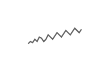
\begin{tikzpicture}[x=0.08em, y=0.08em, line width=0.4pt]
                \draw[FooterGray] (0,3) -- (1,4) -- (2,3.5) -- (3,5) -- (4,4) -- (5,6) -- (6,5.5) -- (7,4) -- (8,5) -- (9,7) -- (10,6) -- (11,5) -- (12,6.5) -- (13,8) -- (14,7) -- (15,6) -- (16,7.5) -- (17,9) -- (18,8) -- (19,7) -- (20,8.5) -- (21,10) -- (22,9) -- (23,8) -- (24,9.5);
            \end{tikzpicture}%
        }%
        \hskip0.5cm%
    }%
    \vskip6pt%
}

%=============================================================================
% PACHETE
%=============================================================================
\usepackage[utf8]{inputenc}
\usepackage[T1]{fontenc}
\usepackage{amsmath, amssymb, amsthm}
\usepackage{mathtools}
\usepackage{bm}
\usepackage{tikz}
\usetikzlibrary{arrows.meta, positioning, shapes, calc, decorations.pathreplacing, shadings}
\usepackage{booktabs}
\usepackage{multirow}
\usepackage{array}
\usepackage{graphicx}
\usepackage{hyperref}
\usepackage{colortbl}
\usepackage{pifont}
\hypersetup{colorlinks=true, linkcolor=MainBlue, urlcolor=MainBlue}
\graphicspath{{../../logos/}{../../charts/}{../../photos/}}
\hfuzz=2pt  % Suppress tiny overfull warnings (<2pt)
\vfuzz=2pt  % Suppress tiny vertical overfull warnings (<2pt)

%=============================================================================
% COMANDA QUANTLET
%=============================================================================
\newcommand{\quantlet}[2]{%
    \vspace{-0.25cm}%
    \hfill\href{#2}{%
        \raisebox{-0.15em}{
\includegraphics[height=0.7em]{ql_logo.png}}%
        \textcolor{MainBlue}{\tiny\ #1}%
    }\par%
}

%=============================================================================
% PAGINĂ TITLU PERSONALIZATĂ
%=============================================================================
\defbeamertemplate*{title page}{hybrid}[1][]
{
    \vspace{0.2cm}
    % Rând logo-uri - antet superior (cu linkuri clickabile)
    \begin{center}
        \href{https://www.ase.ro}{
\includegraphics[height=1.0cm]{ase_logo.png}}\hspace{0.3cm}%
        \href{https://theida.net}{
\includegraphics[height=1.0cm]{ida_logo.png}}\hspace{0.3cm}%
        \href{https://blockchain-research-center.com}{
\includegraphics[height=1.0cm]{brc_logo.png}}\hspace{0.3cm}%
        \href{https://www.ai4efin.ase.ro}{
\includegraphics[height=1.0cm]{ai4efin_logo.png}}\hspace{0.3cm}%
        \href{https://ipe.ro/new}{
\includegraphics[height=1.0cm]{acad_logo.png}}\hspace{0.3cm}%
        \href{https://www.digital-finance-msca.com}{
\includegraphics[height=1.0cm]{msca_logo.png}}%
    \end{center}

    \vspace{0.6cm}

    % Titlu principal cu logo-uri Q pe părți (cu linkuri clickabile)
    \begin{center}
        \begin{minipage}{0.1\textwidth}
            \centering
            \href{https://quantlet.com}{
\includegraphics[height=1.1cm]{ql_logo.png}}
        \end{minipage}%
        \begin{minipage}{0.78\textwidth}
            \centering
            {\LARGE\bfseries\usebeamercolor[fg]{title}\inserttitle}

            \vspace{0.3cm}

            {\usebeamerfont{subtitle}\usebeamercolor[fg]{title}\insertsubtitle}
        \end{minipage}%
        \begin{minipage}{0.1\textwidth}
            \centering
            \href{https://quantinar.com}{
\includegraphics[height=1.1cm]{qr_logo.png}}
        \end{minipage}
    \end{center}

    \vspace{0.6cm}

    % Autori (aliniere la stânga)
    \hspace{0.5cm}\begin{minipage}[t]{0.9\textwidth}
        \usebeamerfont{author}\insertauthor
    \end{minipage}

    \vspace{0.3cm}

    % Institut/Afilieri (aliniere la stânga)
    \hspace{0.5cm}\begin{minipage}[t]{0.9\textwidth}
        \raggedright\small\insertinstitute
    \end{minipage}
}

%=============================================================================
% MEDII PENTRU TEOREME
%=============================================================================
\theoremstyle{definition}
\setbeamertemplate{theorems}[numbered]
\newtheorem{defn}{Definiție}
\newtheorem{thm}{Teoremă}
\newtheorem{prop}{Propoziție}
\newtheorem{rmk}{Observație}

%=============================================================================
% CENTRED MINIPAGE
%=============================================================================
\newenvironment{cminipage}[1]{%
    \par\noindent\hfill\begin{minipage}{#1}\ignorespaces
}{%
    \end{minipage}\hfill\null\par
}

%=============================================================================
% COMENZI PERSONALIZATE
%=============================================================================
\newcommand{\E}{\mathbb{E}}
\newcommand{\Var}{\text{Var}}
\newcommand{\Cov}{\text{Cov}}
\newcommand{\Corr}{\text{Corr}}
\newcommand{\R}{\mathbb{R}}
\newcommand{\N}{\mathbb{N}}
\newcommand{\Z}{\mathbb{Z}}
\newcommand{\B}{\mathbf{B}}
\newcommand{\imark}{\textcolor{MainBlue}{\textbullet}}
\newcommand{\RMSE}{\text{RMSE}}
\newcommand{\MAE}{\text{MAE}}
\newcommand{\MAPE}{\text{MAPE}}

% Indicatoare nivel academic pe slide-uri  (numeric \ifnum — bulletproof in beamer templates)
\newcount\slidelevelnum
\global\slidelevelnum=0
\makeatletter
\newcommand{\slidelevel}[1]{%
    \global\slidelevelnum=0%
    \def\tmp@SL{#1}\def\tmp@SLy{Y3}\def\tmp@SLm{MSc}\def\tmp@SLp{PhD}%
    \ifx\tmp@SL\tmp@SLy \global\slidelevelnum=1\fi%
    \ifx\tmp@SL\tmp@SLm \global\slidelevelnum=2\fi%
    \ifx\tmp@SL\tmp@SLp \global\slidelevelnum=3\fi%
}
\makeatother
\gdef\currentlevelcolor{FooterGray}
\newcommand{\showlevel}{%
    \ifnum\slidelevelnum=1%
        \colorbox{Forest}{\strut\textcolor{white}{\sffamily\bfseries\fontsize{8}{9}\selectfont Y3}}%
        \gdef\currentlevelcolor{Forest}%
    \fi%
    \ifnum\slidelevelnum=2%
        \colorbox{MainBlue}{\strut\textcolor{white}{\sffamily\bfseries\fontsize{8}{9}\selectfont MSc}}%
        \gdef\currentlevelcolor{MainBlue}%
    \fi%
    \ifnum\slidelevelnum=3%
        \colorbox{Crimson}{\strut\textcolor{white}{\sffamily\bfseries\fontsize{8}{9}\selectfont PhD}}%
        \gdef\currentlevelcolor{Crimson}%
    \fi%
    \ifnum\slidelevelnum=0%
        \gdef\currentlevelcolor{FooterGray}%
    \fi%
}


%=============================================================================
% INFORMATII TITLU
%=============================================================================
\title[Statistica Piețelor Financiare]{Statistica Piețelor Financiare}
\subtitle{Capitolul 3: Distribuții cu cozi grele și teoria valorilor extreme}
\author[D.T. Pele, A. Amza]{\texorpdfstring{\begin{tabular}[t]{@{}l@{}}Daniel Traian PELE \\ Antoaneta Amza\end{tabular}}{Daniel Traian PELE, Antoaneta Amza}}
\institute{Academia de Studii Economice din București\\
IDA Institute Digital Assets\\
Blockchain Research Center\\
AI4EFin Artificial Intelligence for Energy Finance\\
Academia Română, Institutul de Prognoză Economică\\
MSCA Digital Finance}
\date{}

\begin{document}

% Pagina de titlu (fara antet/subsol)
{
\setbeamertemplate{headline}{}
\setbeamertemplate{footline}{}
\begin{frame}
    \titlepage
\end{frame}
}

%=============================================================================
% OBIECTIVE DE INVATARE
%=============================================================================
\begin{frame}{Obiective de învățare}
    \begin{block}{La sfârșitul acestui curs, veți fi capabili să:}
    \begin{enumerate}
        \item[\textcolor{MainBlue}{\textbf{1.}}] \textbf{Explicați} rolul distribuțiilor asimetrice (skew-$t$, GED) în modelarea financiară
        \item[\textcolor{MainBlue}{\textbf{2.}}] \textbf{Interpretați} parametrii distribuțiilor $\alpha$-stabile și implicațiile lor
        \item[\textcolor{MainBlue}{\textbf{3.}}] \textbf{Aplicați} Teorema Limită Centrală Generalizată și distribuțiile stabile
        \item[\textcolor{MainBlue}{\textbf{4.}}] \textbf{Utilizați} Teoria Valorilor Extreme (GEV, GPD, metoda POT)
        \item[\textcolor{MainBlue}{\textbf{5.}}] \textbf{Calculați} VaR și ES bazate pe EVT
    \end{enumerate}
    \end{block}
\end{frame}

%=============================================================================
% CUPRINS
%=============================================================================
{
\setbeamertemplate{headline}{%
    \vskip10pt%
    \hbox to \paperwidth{\hskip0.5cm\hfill\hskip0.5cm}%
    \vskip4pt%
    {\color{FooterGray}\hrule height 0.4pt}%
}
\begin{frame}{}
    {\color{FooterGray}\hrule height 0.4pt}
    \vspace{0.1cm}
    {\Large\textcolor{IDAred}{\textbf{Cuprins}}}
    \vspace{0.2cm}
    {\small
    \begin{itemize}
        \item Distribuții asimetrice
        \item Distribuții stabile ($\alpha$-stabile)
        \item Teoria Valorilor Extreme (EVT)
    \end{itemize}
    }
\end{frame}
}

%=============================================================================
% TITLU PARTEA I
\section{Distribuții asimetrice}

%--- Y3 Slide 1 ---
\slidelevel{Y3}
\begin{frame}{De ce contează asimetria}
\begin{itemize}
\item Asimetrie negativă în randamentele acțiunilor: riscul descendent este mai mare decât potențialul ascendent
\item \textbf{Asimetria} măsoară lipsa de simetrie: $S = \E[(X-\mu)^3]/\sigma^3$
\item Distribuțiile simetrice (normală, Student-$t$) atribuie probabilitate egală cozii stângi și drepte
\item Dar empiric: coada stângă a randamentelor acțiunilor este \textbf{mai grea} decât cea dreaptă
\item Avem nevoie de distribuții care pot distinge comportamentul cozii stângi de cel al cozii drepte
\end{itemize}

\vspace{0.3cm}
\begin{alertblock}{Implicație pentru risc}
\begin{itemize}
\item Ignorarea asimetriei duce la subestimarea \textbf{riscului descendent}
\item Un model simetric cu kurtosis corectă alocă totuși greșit probabilitatea între cele două cozi
\end{itemize}
\end{alertblock}
\end{frame}

%--- Y3 Slide 2 ---
\slidelevel{Y3}
\begin{frame}{Asimetria în randamentele financiare}
\begin{center}
\renewcommand{\arraystretch}{1.1}
\begin{tabular}{lcc}
\toprule
\textbf{Clasă de active} & \textbf{Asimetrie tipică} & \textbf{Implicație} \\
\midrule
Indici de acțiuni & $-0{,}1$ la $-0{,}5$ & Coada stângă mai grea \\
Acțiuni individuale & $-0{,}3$ la $-1{,}0$ & Risc mare de prăbușire \\
FX majore & $\approx 0$ & Aproximativ simetrică \\
Mărfuri & Mixt & Depinde de șocurile de ofertă \\
Obligațiuni & Ușor pozitivă & Coada dreaptă (salturi de randament) \\
\bottomrule
\end{tabular}
\end{center}

\vspace{0.2cm}
\begin{itemize}
\item Asimetria afectează VaR 1\%: o distribuție asimetrică la stânga are o cuantilă stângă mai extremă decât o distribuție simetrică cu aceeași varianță
\end{itemize}
\end{frame}

%--- MSc Slide 3 ---
\slidelevel{MSc}
\begin{frame}{Distribuția Student-$t$ asimetrică (Hansen)}
\begin{defn}[Student-$t$ asimetrică Hansen (Hansen, 1994)]
\[
f(x;\nu,\lambda) = \begin{cases}
bc\!\left(1 + \frac{1}{\nu-2}\left(\frac{bx+a}{1-\lambda}\right)^{\!2}\right)^{-(\nu+1)/2} & x < -a/b \\[6pt]
bc\!\left(1 + \frac{1}{\nu-2}\left(\frac{bx+a}{1+\lambda}\right)^{\!2}\right)^{-(\nu+1)/2} & x \geq -a/b
\end{cases}
\]
unde $\lambda \in (-1,1)$ este parametrul de asimetrie, $a = 4\lambda c\frac{\nu-2}{\nu-1}$, $b^2 = 1 + 3\lambda^2 - a^2$, $c = \frac{\Gamma((\nu+1)/2)}{\sqrt{\pi(\nu-2)}\,\Gamma(\nu/2)}$.
\end{defn}

\begin{itemize}
\item $\lambda = 0$: Student-$t$ simetrică; \quad $\lambda < 0$: coada stângă mai grea
\item Comportament asimptotic: coada stângă $\sim |x|^{-\nu-1}(1-\lambda)^{\nu+1}$, coada dreaptă $\sim x^{-\nu-1}(1+\lambda)^{\nu+1}$
\item $\lambda < 0$ $\Rightarrow$ coada stângă mai grea (risc de pierdere mai mare)
\item Utilizată frecvent ca distribuție a inovațiilor GARCH
\end{itemize}
\end{frame}

%--- MSc Slide 3b ---
\slidelevel{MSc}
\begin{frame}{Densitățile skew-$t$ --- Efectul parametrului $\lambda$}
\begin{center}
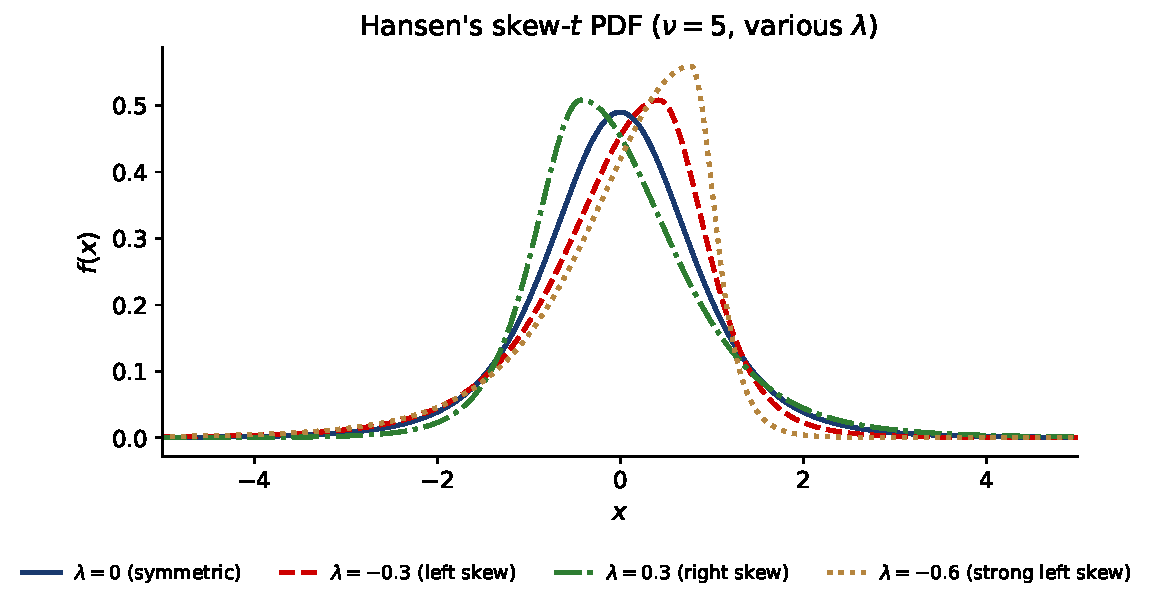
\includegraphics[width=0.58\textwidth]{ch2_skew_t_pdf_theoretical.pdf}
\end{center}
\begin{itemize}
\item $\lambda < 0$: coada \textbf{stângă} mai grea (tipic pentru acțiuni)
\item $\lambda > 0$: coada \textbf{dreaptă} mai grea
\item Cu cât $|\lambda|$ este mai mare, cu atât asimetria este mai pronunțată
\end{itemize}
\end{frame}

%--- MSc Slide 4 ---
\slidelevel{MSc}
\begin{frame}{Distribuția erorilor generalizate (GED)}
\begin{defn}[GED --- forma standardizată]
\[
f(x;\nu) = \frac{\nu}{2\lambda\,\Gamma(1/\nu)}\exp\!\left(-\left|\frac{x}{\lambda}\right|^\nu\right), \quad \nu > 0,
\]
unde $\lambda = \sqrt{2^{-2/\nu}\,\Gamma(1/\nu)\,/\,\Gamma(3/\nu)}$ asigură $\Var(X) = 1$.
\end{defn}

\begin{itemize}
\item $\nu = 2$: distribuția normală; \quad $\nu = 1$: Laplace (exponențială dublă)
\item $\nu < 2$: cozi mai groase decât distribuția normală; \quad $\nu > 2$: cozi mai subțiri
\item Controlează grosimea cozilor printr-un singur parametru
\item Populară în modele GARCH: GARCH-GED
\end{itemize}

\vspace{0.2cm}
\begin{block}{Estimare MLE}
\begin{itemize}
\item Atât pentru Student-$t$ asimetrică cât și pentru GED, parametrii se estimează prin verosimilitate maximă
\item Se compară prin AIC/BIC
\end{itemize}
\end{block}
\end{frame}

%--- MSc Slide 5 ---
\slidelevel{MSc}
\begin{frame}{Compararea distribuțiilor asimetrice}
\begin{center}
\renewcommand{\arraystretch}{1.1}
\begin{tabular}{lccc}
\toprule
\textbf{Distribuție} & \textbf{Parametri} & \textbf{Asimetrie} & \textbf{Tip coadă} \\
\midrule
Normală & $\mu, \sigma$ & 0 & Exponențială \\
Student-$t$ & $\mu, \sigma, \nu$ & 0 & Lege putere \\
Student-$t$ asim. & $\mu, \sigma, \nu, \lambda$ & $\neq 0$ & Lege putere (asim.) \\
GED & $\mu, \sigma, \nu$ & 0 & Exponențială generalizată \\
NIG & $\alpha, \beta, \delta, \mu$ & $\neq 0$ & Semi-grea \\
\bottomrule
\end{tabular}
\end{center}

\begin{itemize}
\item Mai mulți parametri $\Rightarrow$ ajustare mai bună dar risc de supraajustare
\item AIC/BIC echilibrează calitatea ajustării cu complexitatea
\item Pentru randamente zilnice de acțiuni: Student-$t$ asimetrică domină adesea
\end{itemize}
\end{frame}

%--- PhD Slide 6 ---
\slidelevel{PhD}
\begin{frame}{Familia hiperbolică generalizată}
\begin{itemize}
\item Distribuția \textbf{hiperbolică generalizată (GH)}: cinci parametri $(\lambda, \alpha, \beta, \delta, \mu)$
\item PDF:
\[
f(x) \propto \left(\delta^2 + (x-\mu)^2\right)^{(\lambda - 1/2)/2} K_{\lambda-1/2}\!\left(\alpha\sqrt{\delta^2 + (x-\mu)^2}\right) e^{\beta(x-\mu)}
\]
unde $K_\nu$ este funcția Bessel modificată de speța a doua
\item Cazuri speciale:
\begin{itemize}
\item \textbf{Hiperbolică}: $\lambda = 1$
\item \textbf{NIG} (Normal Inverse Gaussiană): $\lambda = -1/2$
\item \textbf{VG} (Variance Gamma): $\delta \to 0$
\end{itemize}
\end{itemize}
\end{frame}

%--- PhD Slide 7 ---
\slidelevel{PhD}
\begin{frame}{Mixturi normale medie-varianță}
\begin{itemize}
\item \textbf{GH ca mixtură normală medie-varianță}:
\[
X \mid W \sim N(\mu + \beta W, W), \quad W \sim \text{GIG}(\lambda, \delta, \gamma)
\]
unde GIG este distribuția Gaussiană Inversă Generalizată
\item Barndorff-Nielsen (1977): ajustare empirică excelentă pe date financiare
\item \textbf{Închidere afină}: distribuțiile GH sunt închise la transformări afine
\item GH multivariată: tratabilă pentru probleme de portofoliu
\item Conexiunea cu procesele L\'{e}vy: distribuțiile GH sunt infinit divizibile $\Rightarrow$ procese L\'{e}vy GH
\end{itemize}

\begin{rmk}[De ce contează?]
\begin{itemize}
\item Familia GH este utilizată pe scară largă în managementul riscului de portofoliu
\item Deutsche Bank, JP Morgan și alte instituții o folosesc pentru modelarea multivariată a randamentelor
\item Cazul special NIG oferă cel mai bun compromis precizie/tratabilitate
\end{itemize}
\end{rmk}
\end{frame}

%--- Y3 Slide 8 ---
\slidelevel{Y3}
\begin{frame}{Vizualizarea asimetriei --- Date reale S\&P 500}
\vspace{-0.2cm}
\begin{center}
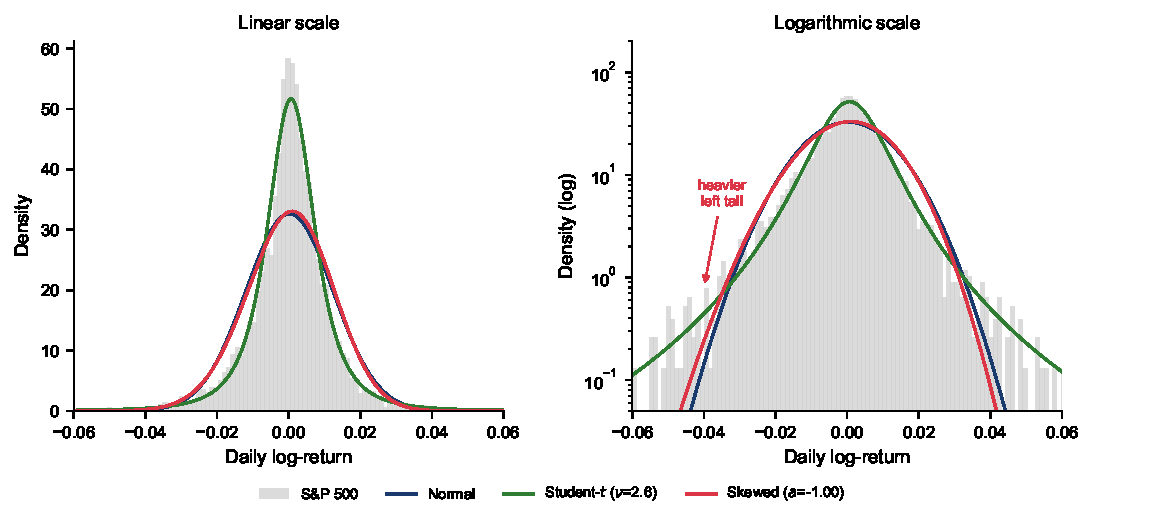
\includegraphics[width=0.75\linewidth]{ch2_skew_t_densities.pdf}
\end{center}
\quantlet{SFM\_ch2\_skew\_t}{https://github.com/QuantLet/Stat_fin_markets/tree/master/Ch_02/SFM_ch2_asymmetric_distributions}
\vspace{-0.4cm}
\begin{itemize}\setlength\itemsep{0pt}
\item Pe \textbf{scală logaritmică}, diferențele în cozi devin vizibile
\item Coada stângă: asimetrică $>$ Student-$t$ $\gg$ normală $\Rightarrow$ VaR subestimat fără asimetrie
\end{itemize}
\end{frame}

%--- Y3 Slide 9 ---
\slidelevel{Y3}
\begin{frame}{Exemplu: Impactul asimetriei asupra VaR}
\begin{exampleblock}{Exercițiu}
Portofoliu \$1M, $\sigma\!=\!1{,}5\%$, $\nu\!=\!5$. VaR 1\%: Student-$t$ simetrică ($\lambda\!=\!0$) vs.\ asim.\ ($\lambda\!=\!-0{,}3$).
\end{exampleblock}

\begin{block}{Rezolvare}
\begin{center}
\renewcommand{\arraystretch}{1.1}
\begin{tabular}{lccc}
\toprule
\textbf{Model} & $z_{0{,}01}$ & VaR 1\% & \textbf{\$ pierdere} \\
\midrule
Normal & $-2{,}326$ & $3{,}49\%$ & \$34.890 \\
Student-$t$ sim.\ ($\nu\!=\!5$) & $-3{,}365$ & $5{,}05\%$ & \$50.475 \\
Student-$t$ asim.\ ($\lambda\!=\!-0{,}3$) & $-3{,}87$ & $5{,}81\%$ & \$58.050 \\
\bottomrule
\end{tabular}
\end{center}

\begin{itemize}
\item Trecerea de la simetrică la asimetrică crește VaR cu \textbf{15\%}
\item Asimetria negativă ,,deplasează'' masă probabilistică spre pierderi mari
\item \textbf{Capitalul necesar} crește cu \$7.575 doar din efectul asimetriei
\end{itemize}
\end{block}
\end{frame}

%=============================================================================
% SECȚIUNEA 7: DISTRIBUȚII STABILE
%=============================================================================
\section{Distribuții stabile ($\alpha$-stabile)}

%--- Y3 Slide 1 ---
\slidelevel{Y3}
\begin{frame}{Ce este o distribuție stabilă?}
\begin{defn}[Distribuție stabilă --- Intuitiv]
O distribuție este \textbf{stabilă} dacă suma de copii i.i.d.\ are aceeași formă (până la locație și scală). Formal, $X \sim S(\alpha, \beta, \gamma, \delta)$ dacă pentru copii i.i.d.\ $X_1, X_2$:
\[
aX_1 + bX_2 \stackrel{d}{=} cX + d, \quad c = (a^\alpha + b^\alpha)^{1/\alpha}.
\]
\end{defn}

\begin{itemize}
\item \textbf{Patru parametri}:
\begin{itemize}
\item $\alpha \in (0, 2]$: \textbf{indicele de stabilitate} (grosimea cozilor) --- $\alpha$ mai mic $\Rightarrow$ cozi mai groase
\item $\beta \in [-1, 1]$: \textbf{asimetrie}
\item $\gamma > 0$: \textbf{scală}
\item $\delta \in \R$: \textbf{locație}
\end{itemize}
\item Cazuri speciale: $\alpha = 2$ (Gaussiană), $\alpha = 1, \beta = 0$ (Cauchy)
\end{itemize}
\end{frame}

%--- Y3 Slide 1b ---
\slidelevel{Y3}
\begin{frame}{Densitățile $\alpha$-stabile --- Efectul lui $\alpha$}
\vspace{-0.2cm}
\begin{center}
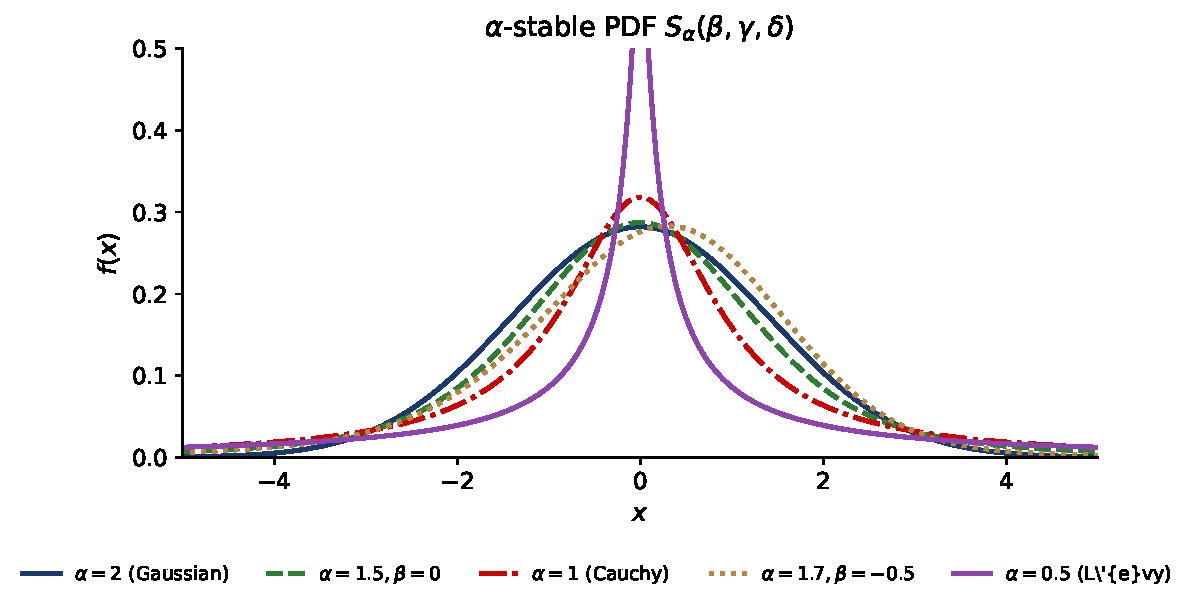
\includegraphics[width=0.52\textwidth]{ch2_stable_pdf_theoretical.pdf}
\end{center}
\vspace{-0.2cm}
\begin{itemize}
\item $\alpha = 2$: \textbf{Gaussiană}; \quad $\alpha < 2$: cozi \textbf{lege putere (\textit{power law})} $f(x) \sim |x|^{-(1+\alpha)}$
\item $\alpha = 1$: \textbf{Cauchy} ($\E[|X|] = \infty$); \quad $\beta \neq 0$: introduce \textbf{asimetrie}
\end{itemize}
\end{frame}

%--- Y3 Slide 2 ---
\slidelevel{Y3}
\begin{frame}{De ce varianța poate să nu existe}
\begin{itemize}
\item Pentru $\alpha < 2$: $\E[|X|^p] < \infty$ dacă și numai dacă $p < \alpha$
\item În particular, $\E[X^2] = \infty$ când $\alpha < 2$ --- \textbf{varianța nu există}
\item Varianța eșantionului nu converge la o constantă; crește odată cu $n$
\item \textbf{Mandelbrot (1963)}: variațiile prețului bumbacului urmează legi stabile cu $\alpha \approx 1{,}7$
\item Estimări tipice pentru randamente financiare: $\hat{\alpha} \in [1{,}5;\ 1{,}9]$
\end{itemize}
\end{frame}

%--- Y3 Slide 2b ---
\slidelevel{Y3}
\begin{frame}{Varianța eșantionului --- convergență vs.\ divergență}
\vspace{-0.1cm}
\begin{center}
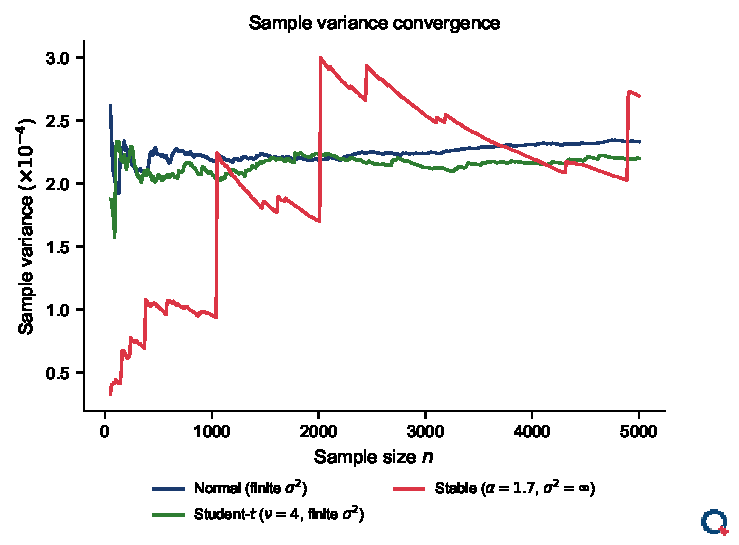
\includegraphics[width=0.4\textwidth]{ch2_sample_var_diverge.pdf}
\end{center}
\quantlet{SFM\_ch2\_stable\_var}{https://github.com/QuantLet/Stat_fin_markets/tree/master/Ch_02/SFM_ch2_stable_distributions}
\vspace{-0.3cm}
\begin{alertblock}{Schimbare de paradigmă}
\begin{itemize}
\item Dacă $\alpha < 2$, teoria medie-varianță (Markowitz) se prăbușește: varianța nu este o măsură semnificativă de risc
\end{itemize}
\end{alertblock}
\end{frame}

%--- Y3 Slide 3 ---
\slidelevel{Y3}
\begin{frame}{Ajustarea stabilă pe S\&P 500}
\begin{center}
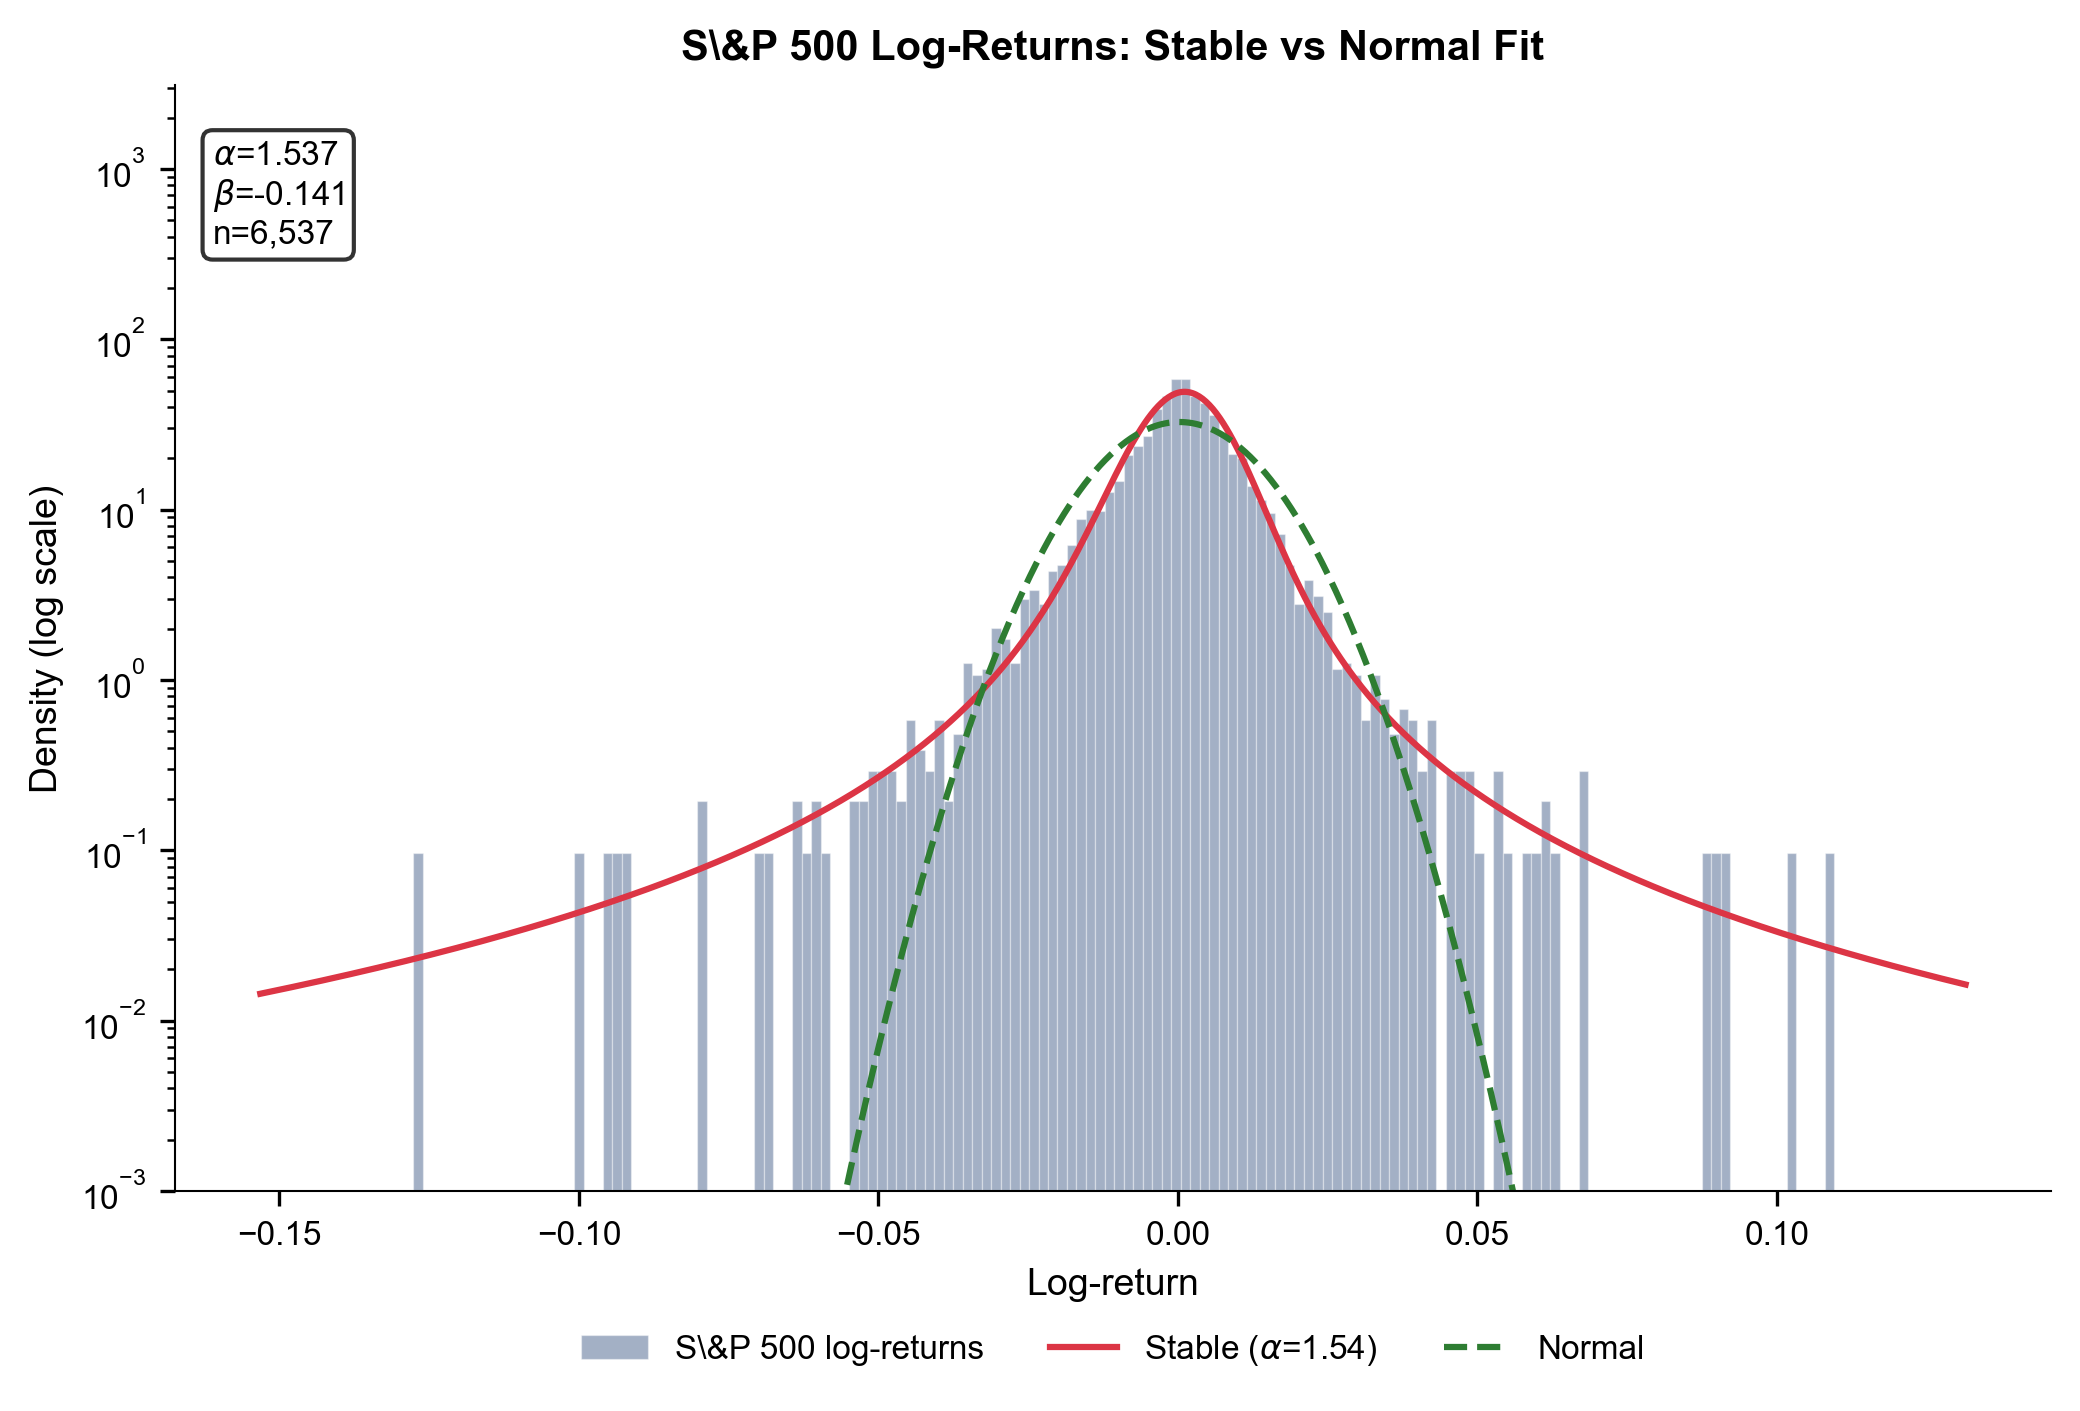
\includegraphics[width=0.5\textwidth]{ch2_sp500_stable_fit.png}
\end{center}
\quantlet{SFM\_ch2\_stable\_fit}{https://github.com/QuantLet/Stat_fin_markets/tree/master/Ch_02/SFM_ch2_stable_distributions}

\begin{itemize}
\item Distribuția stabilă surprinde cozile groase mai bine decât distribuția normală
\item $\hat{\alpha} \approx 1{,}7$ estimat pentru randamentele zilnice S\&P~500
\end{itemize}
\end{frame}

%--- Y3 Slide 4 ---
\slidelevel{Y3}
\begin{frame}{Stabilă vs.\ Normală vs.\ Student-$t$}
\begin{center}
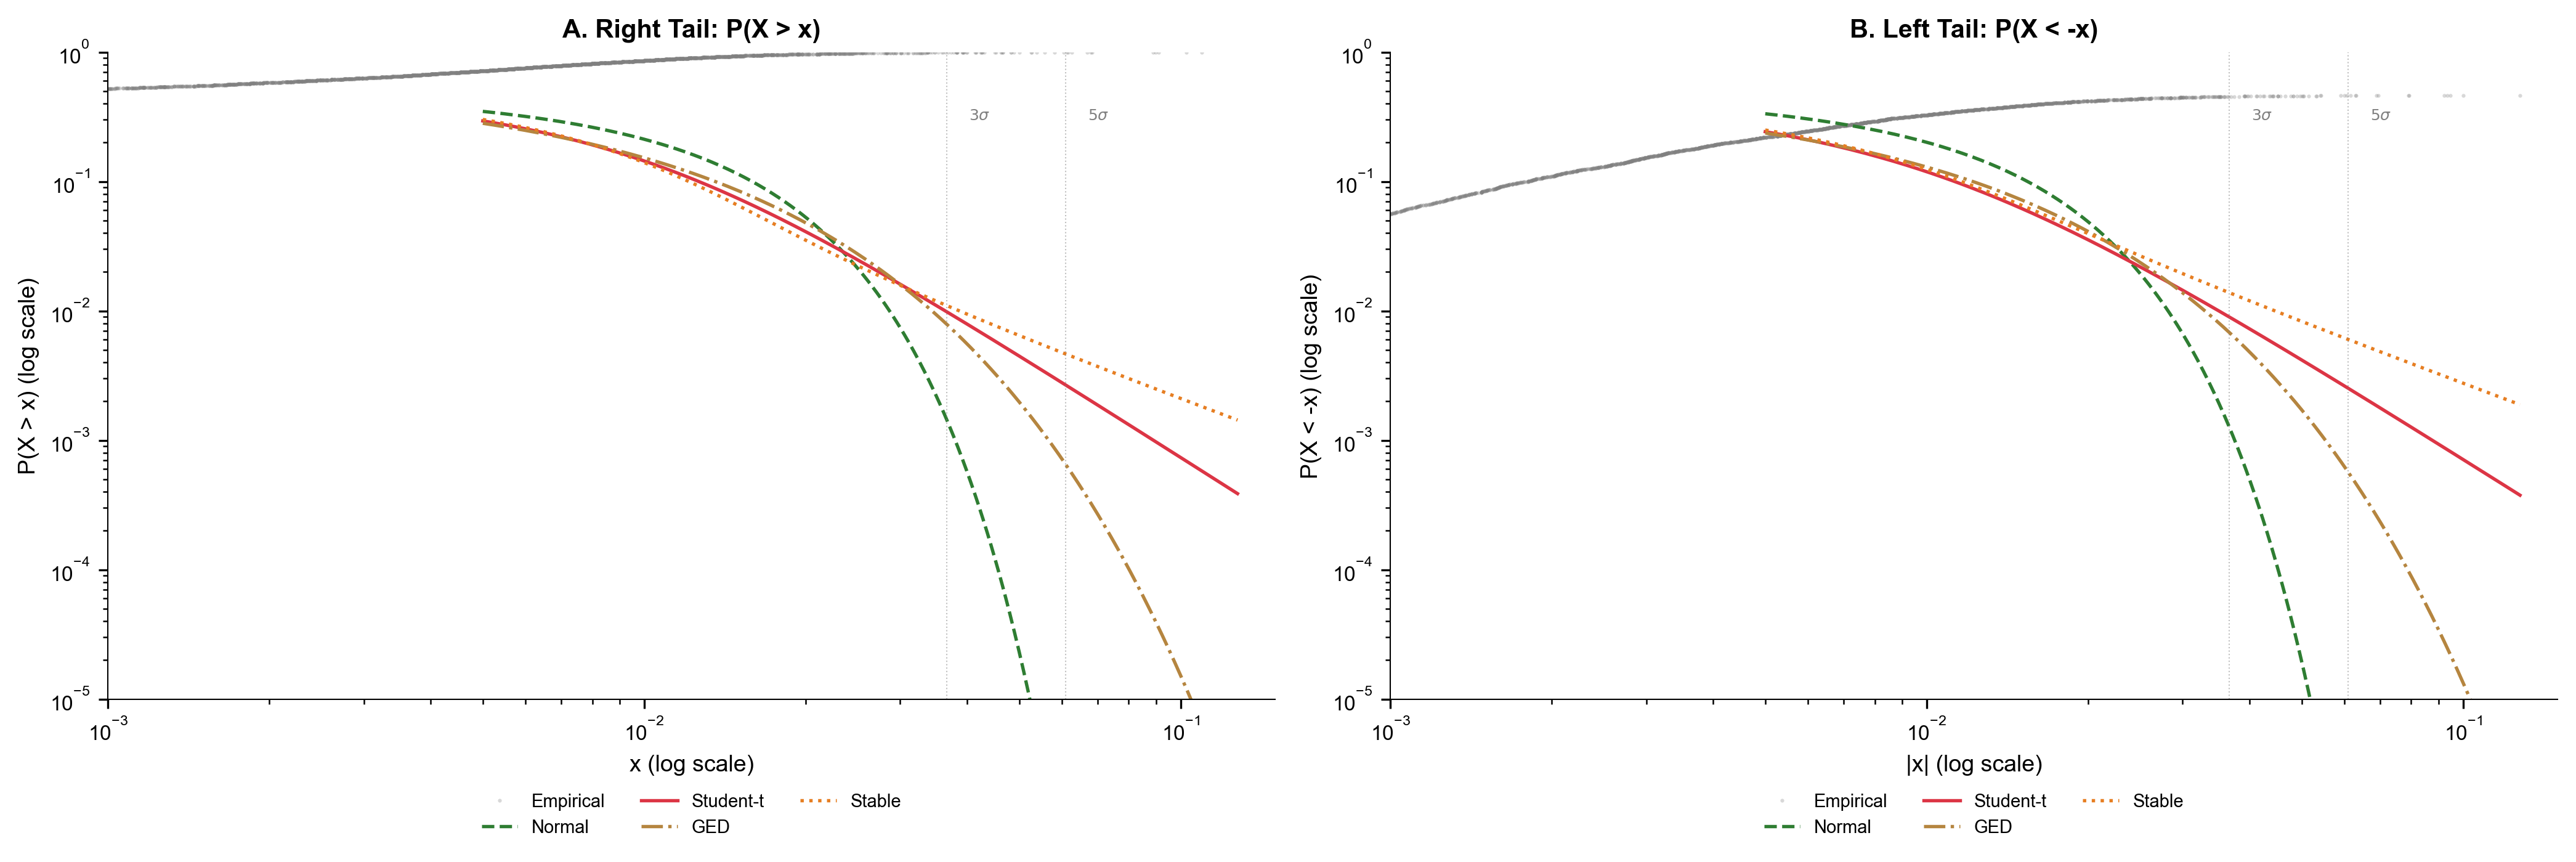
\includegraphics[width=0.65\textwidth]{ch2_dist_comparison_tails.png}
\end{center}
\quantlet{SFM\_ch2\_dist\_tails}{https://github.com/QuantLet/Stat_fin_markets/tree/master/Ch_02/SFM_ch2_distribution_comparison}
\begin{center}
\renewcommand{\arraystretch}{1.1}
\begin{tabular}{lccc}
\toprule
& \textbf{Normală} & \textbf{Student-$t$} & \textbf{Stabilă} \\
\midrule
Descreșterea cozii (PDF) & $e^{-x^2/2}$ & $|x|^{-\nu-1}$ & $|x|^{-\alpha-1}$ \\
Varianța & Finită & Finită ($\nu>2$) & Infinită ($\alpha<2$) \\
Închisă la sumă & Da & Nu & Da \\
Limită TLC & TLC & --- & TLCG \\
\bottomrule
\end{tabular}
\end{center}
\end{frame}

%--- MSc Slide 5 ---
\slidelevel{MSc}
\begin{frame}{Funcția caracteristică}
\begin{itemize}
\item Distribuția stabilă este definită prin \textbf{funcția caracteristică (\textit{characteristic function})} (parametrizarea Nolan $S^1$, $\alpha \neq 1$):
\end{itemize}
\[
\phi(t) = \E[e^{itX}] = \exp\!\left\{-\gamma^\alpha |t|^\alpha\!\left(1 - i\beta\,\text{sign}(t)\tan\frac{\pi\alpha}{2}\right) + i\delta t\right\}
\]
\begin{itemize}
\item Cazul $\alpha = 1$:
\end{itemize}
\[
\phi(t) = \exp\!\left\{-\gamma|t|\!\left(1 + i\beta\frac{2}{\pi}\,\text{sign}(t)\ln|t|\right) + i\delta t\right\}
\]

\begin{itemize}
\item \textbf{Fără PDF în formă închisă} în general (excepții: Gaussiană, Cauchy, L\'{e}vy)
\item Densitatea prin transformata Fourier inversă: $f(x) = \frac{1}{2\pi}\int_{-\infty}^{\infty}\phi(t)\,e^{-itx}\,dt$
\item Evaluare numerică: algoritmul lui Nolan (1997)
\end{itemize}
\begin{rmk}
\begin{itemize}
\item Utilizăm parametrizarea $S^1(\alpha,\beta,\gamma,\delta)$ a lui Nolan (1997) în tot capitolul
\item \texttt{scipy.stats.levy\_stable} folosește parametrizarea $S^0$ --- atenție la conversie!
\end{itemize}
\end{rmk}
\end{frame}

%--- MSc Slide 6 ---
\slidelevel{MSc}
\begin{frame}{Teorema Limită Centrală Generalizată}
\begin{thm}[TLCG]
Distribuțiile stabile sunt singurele limite non-degenerate posibile ale sumelor normalizate:
\[
\frac{S_n - b_n}{a_n} \xrightarrow{d} S(\alpha, \beta, \gamma, \delta)
\]
unde $S_n = X_1 + \cdots + X_n$ pentru $X_i$ i.i.d.
\end{thm}

\begin{itemize}
\item TLC clasică: $\alpha = 2$ (necesită varianță finită)
\item TLCG: $\alpha < 2$ (permite varianță infinită (\textit{infinite variance}))
\item \textbf{Proprietatea de stabilitate}: Sumele de v.a.\ stabile i.i.d.\ rămân stabile cu același $\alpha$
\item \textbf{Cozi tip lege putere}: $P(X > x) \sim C_\alpha(1+\beta)\,x^{-\alpha}$ când $x \to \infty$
\end{itemize}
\end{frame}

%--- MSc Slide 7 ---
\slidelevel{MSc}
\begin{frame}{PDF-uri stabile --- Variind $\alpha$}
\begin{center}
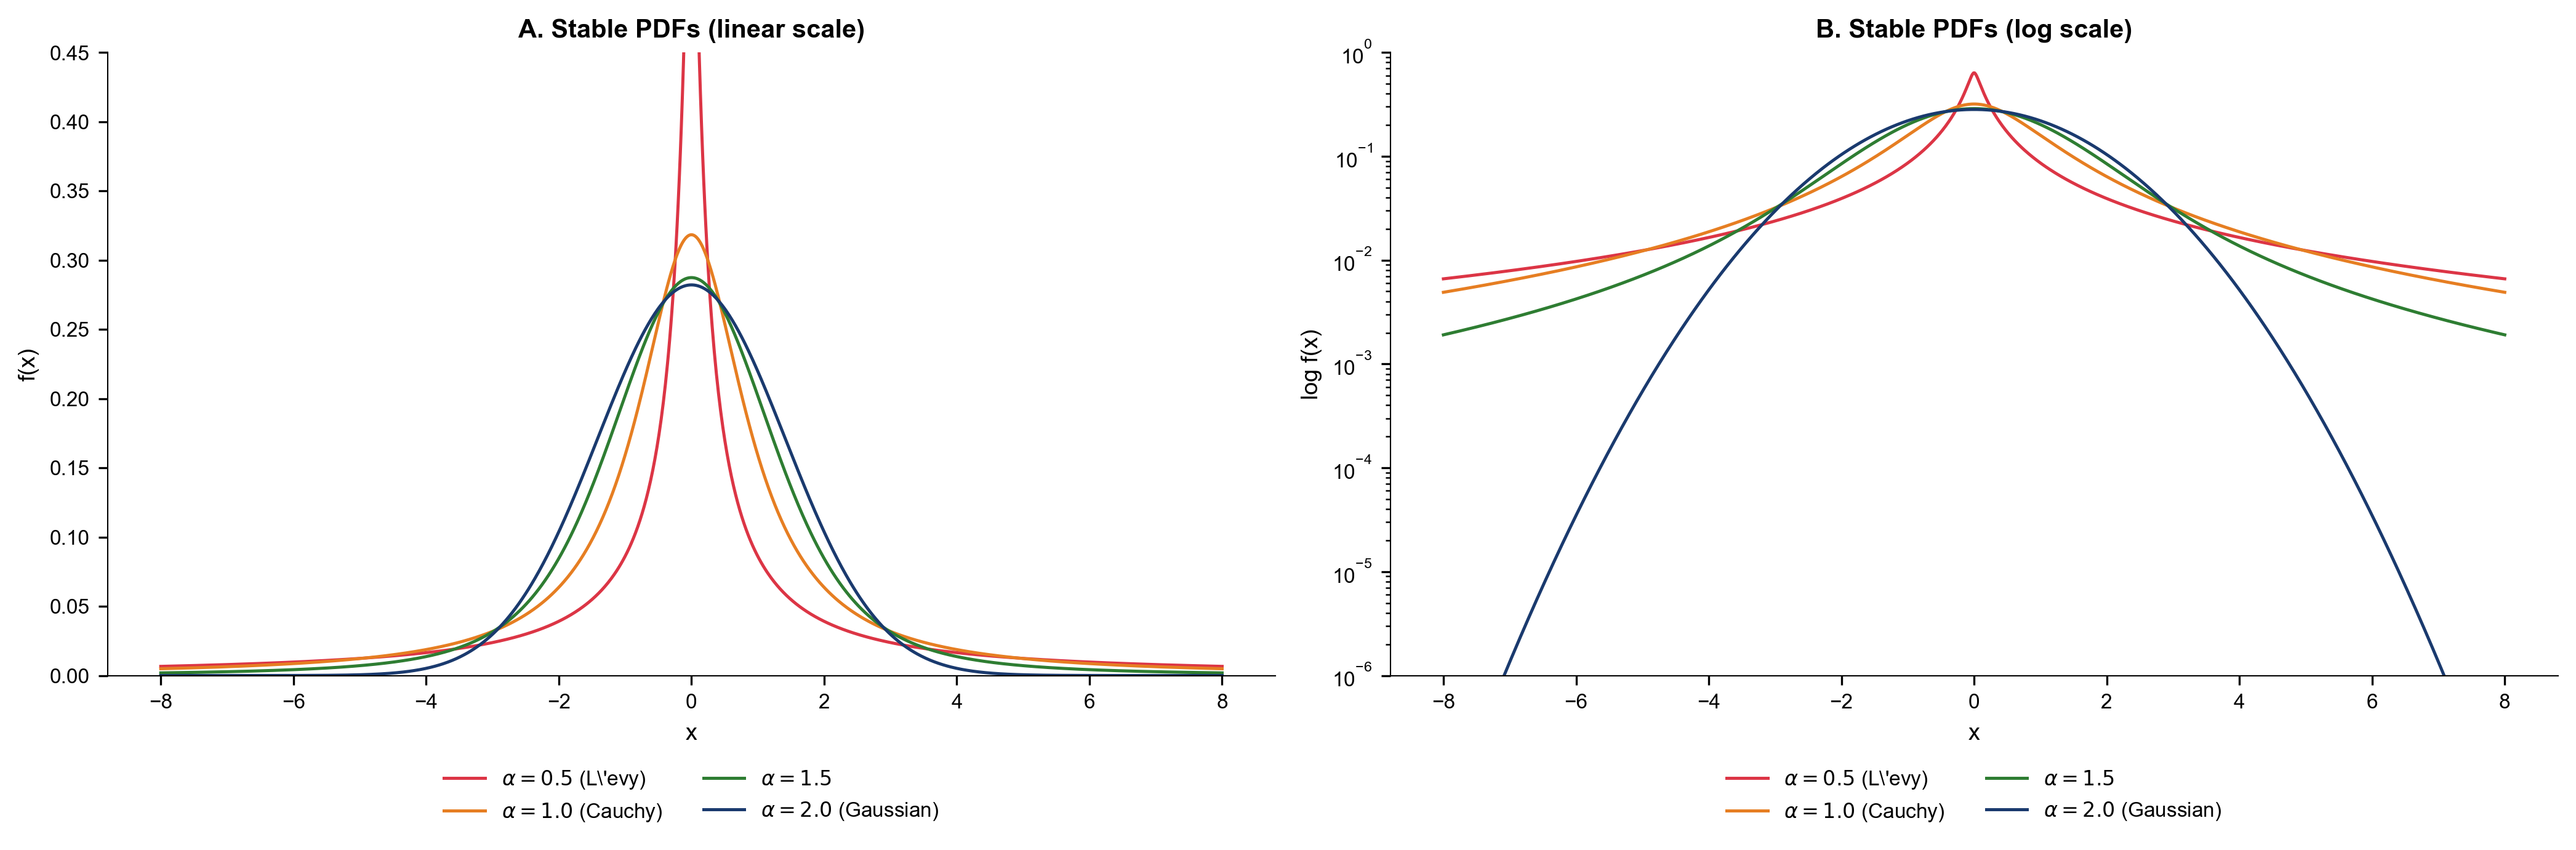
\includegraphics[width=0.72\textwidth]{ch2_stable_pdfs.png}
\end{center}
\quantlet{SFM\_ch2\_stable\_pdfs}{https://github.com/QuantLet/Stat_fin_markets/tree/master/Ch_02/SFM_ch2_stable_distributions}
\begin{itemize}
\item $\alpha$ mai mic $\Rightarrow$ cozi mai groase, vârf mai ascuțit
\item $\alpha = 2$: Gaussiană; $\alpha = 1$: Cauchy
\item Randamente financiare: $\hat{\alpha} \in [1{,}5;\ 1{,}9]$
\end{itemize}
\end{frame}

%--- MSc Slide 8 ---
\slidelevel{MSc}
\begin{frame}{Estimare și analiză cross-asset}
\begin{columns}[T]
\begin{column}{0.48\textwidth}
\begin{block}{Metode de estimare}
\begin{itemize}
\item Metoda cuantilelor McCulloch (rapidă, consistentă)
\item MLE (Nolan, 1997) --- cea mai eficientă
\item Metode bazate pe funcția caracteristică (Kogon \& Williams, 1998)
\end{itemize}
\end{block}
\end{column}
\begin{column}{0.48\textwidth}
\begin{center}
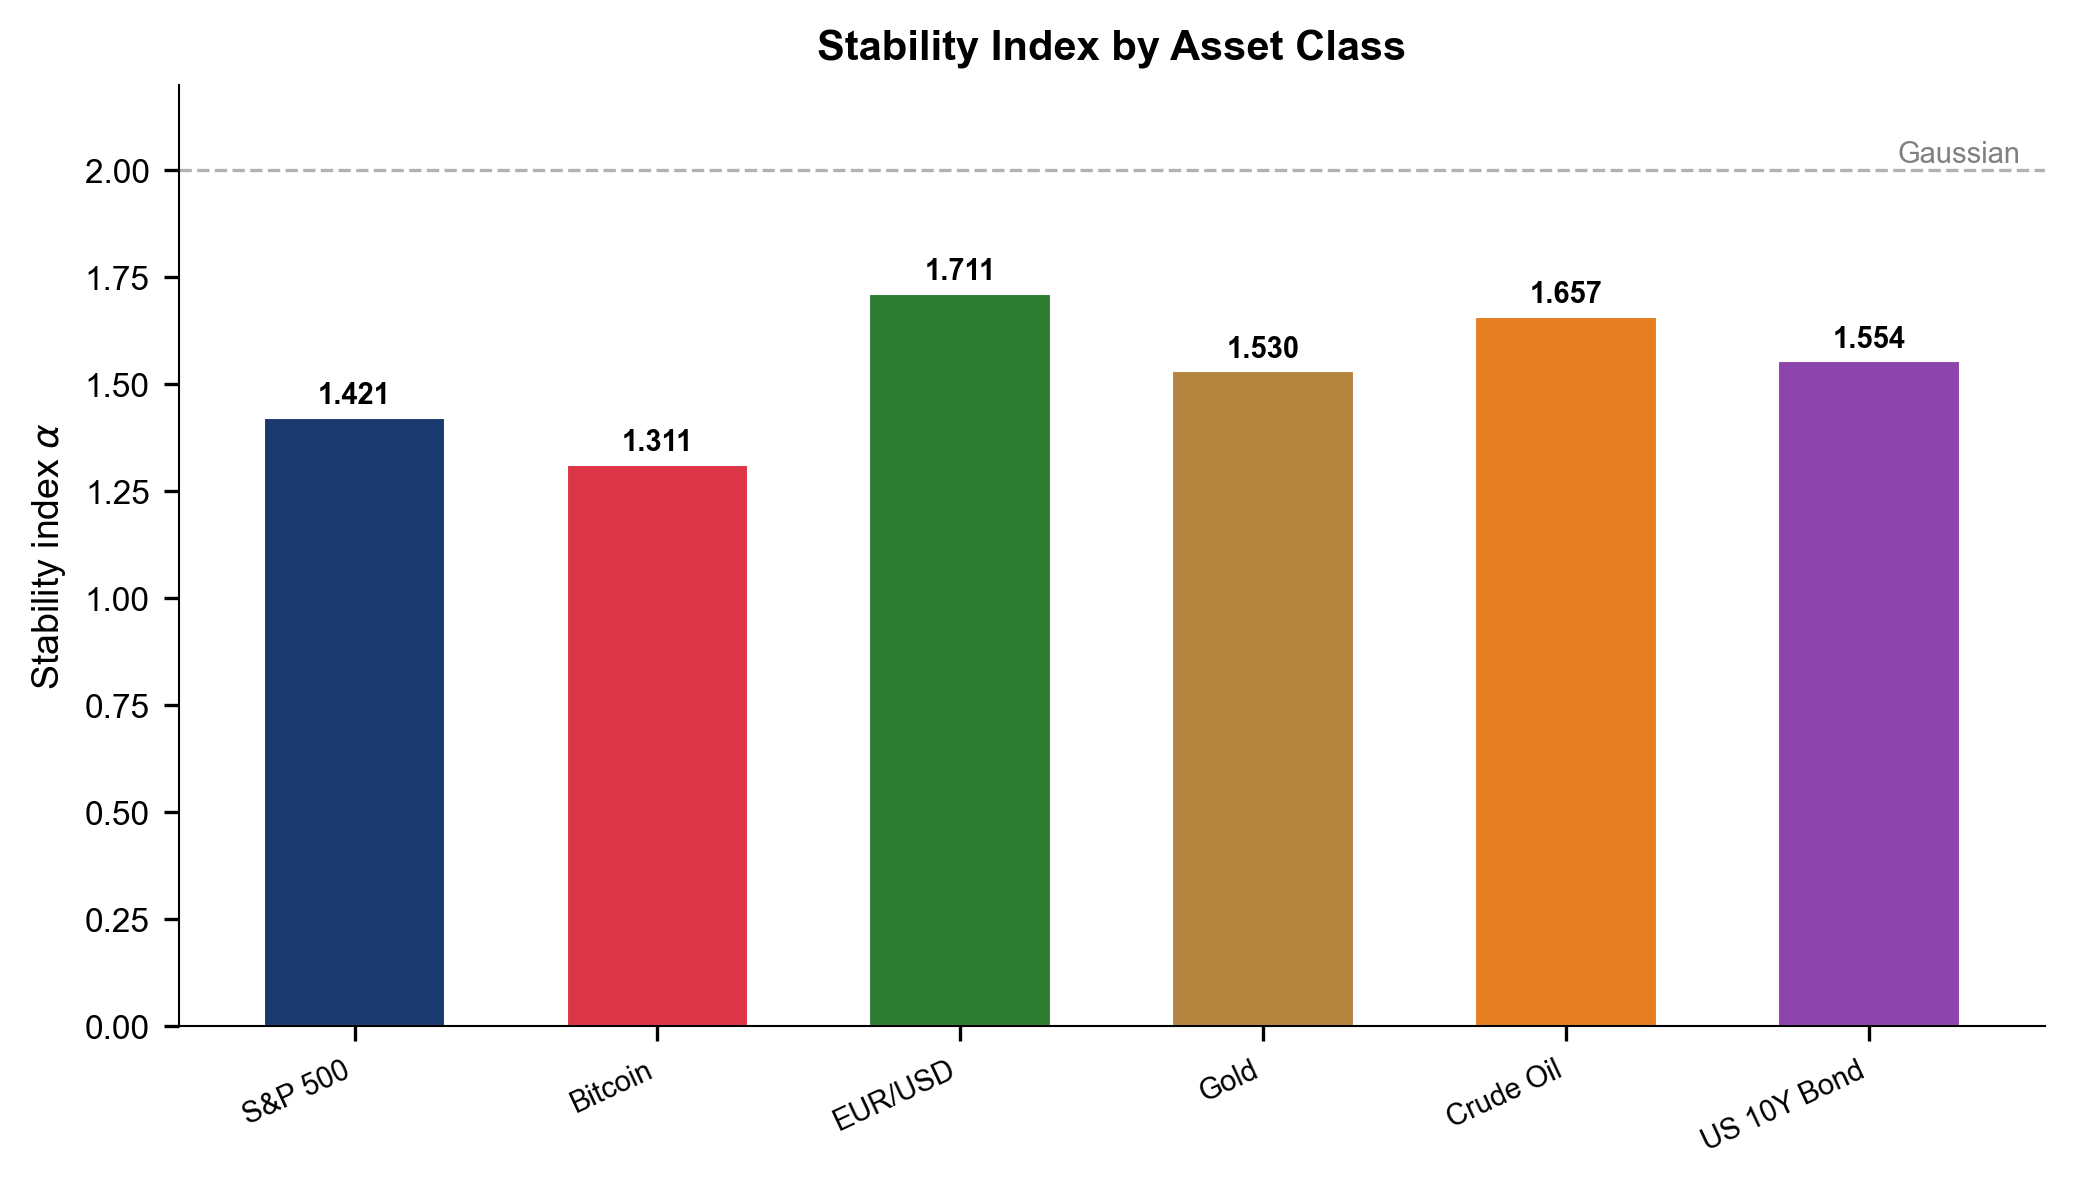
\includegraphics[width=\textwidth]{ch2_cross_asset_alpha.png}
\end{center}
\quantlet{SFM\_ch2\_cross\_asset}{https://github.com/QuantLet/Stat_fin_markets/tree/master/Ch_02/SFM_ch2_stable_distributions}
\end{column}
\end{columns}

\vspace{0.2cm}
\begin{itemize}
\item $\hat{\alpha} \approx 1{,}7$ pentru S\&P~500; $\hat{\alpha} \approx 1{,}5$ pentru Bitcoin; $\hat{\alpha} \approx 1{,}8$ pentru FX
\item $\alpha < 2$ pentru toate clasele majore de active $\Rightarrow$ varianța infinită este ubicuă
\end{itemize}
\end{frame}

%--- PhD Slide 8b ---
\slidelevel{PhD}
\begin{frame}{$\alpha_{\text{stabil}}$ vs.\ $\alpha_{\text{Hill}}$ --- Reconciliere}
\begin{columns}[T]
\begin{column}{0.48\textwidth}
\begin{block}{MLE pe toată distribuția}
\begin{itemize}
\item $\hat{\alpha}_{\text{stabil}} \approx 1{,}7$ (S\&P~500)
\item Captează \textbf{comportamentul global}
\item Include centrul + cozile
\item Implică varianță infinită ($\alpha < 2$)
\end{itemize}
\end{block}
\end{column}
\begin{column}{0.48\textwidth}
\begin{block}{Estimatorul Hill (doar coada)}
\begin{itemize}
\item $\hat{\alpha}_{\text{Hill}} \approx 3\text{--}4$ (S\&P~500)
\item Estimează doar \textbf{indexul de coadă}
\item Folosește doar observațiile extreme
\item Implică varianță finită ($\alpha > 2$)
\end{itemize}
\end{block}
\end{column}
\end{columns}

\vspace{0.1cm}
\begin{alertblock}{Reconciliere: distribuții stabile temperate}
\begin{itemize}
\item Conflictul $\hat{\alpha}_{\text{stabil}} \neq \hat{\alpha}_{\text{Hill}}$ este \textbf{aparent}: cele două estimează cantități diferite
\item Distribuțiile \textbf{stabile temperate} (CGMY) rezolvă paradoxul: comportament stabil pentru $x$ moderat, dar cozi cu decădere exponențial-multiplicată
\item Referințe: McCulloch (1997), Grabchak \& Samorodnitsky (2010)
\end{itemize}
\end{alertblock}
\end{frame}

%--- PhD Slide 9 ---
\slidelevel{PhD}
\begin{frame}{Variație regulată și domeniu de atracție}
\begin{defn}[Variație regulată]
$L : (0,\infty) \to (0,\infty)$ este \textbf{lent variabilă} la infinit dacă $\lim_{x\to\infty} L(tx)/L(x) = 1$ pentru orice $t > 0$. O funcție $f$ este \textbf{regulat variabilă} cu indice $\rho$ dacă $f(x) = x^\rho L(x)$.
\end{defn}

\begin{thm}[Domeniul de atracție]
$F$ aparține domeniului de atracție al $S(\alpha, \beta, 1, 0)$ dacă și numai dacă:
\begin{enumerate}
\item $\bar{F}(x) = x^{-\alpha}L(x)$ (cozi regulat variabile)
\item Condiția de echilibru: $\lim_{x\to\infty} \frac{\bar{F}(x)}{\bar{F}(x) + F(-x)} = \frac{1+\beta}{2}$
\end{enumerate}
\end{thm}

\vspace{0.1cm}
{\small\textit{Variația regulată fundamentează teoria EVT și determină dacă estimatorul Hill este consistent.}}
\end{frame}


%--- PhD Slide 10 ---
\slidelevel{PhD}
\begin{frame}{Procese L\'{e}vy}
\begin{itemize}
\item Un \textbf{proces L\'{e}vy} $\{L_t\}_{t\geq 0}$ are creșteri staționare independente
\item $L_1 \sim S(\alpha, \beta, \gamma, \delta)$ definește un \textbf{proces L\'{e}vy stabil}
\item \textbf{Descompunerea L\'{e}vy--It\^{o}}:
\[
L_t = bt + \sigma W_t + \int_{|x|\leq 1} x\,\tilde{N}(t,dx) + \int_{|x|>1} x\,N(t,dx)
\]
\item \textbf{Măsura L\'{e}vy} a unui proces stabil:
\[
\nu(dx) = \begin{cases} c_+ x^{-\alpha-1}dx & x > 0 \\ c_- |x|^{-\alpha-1}dx & x < 0 \end{cases}
\]
\item Activitate infinită: infinit de multe salturi mici în orice interval finit
\end{itemize}

\begin{rmk}[De ce contează?]
\begin{itemize}
\item Procesele Lévy sunt fundamentul evaluării opțiunilor cu salturi; Black--Scholes $= \nu \equiv 0$
\item Componenta de salt explică zâmbetul volatilității (\textit{volatility smile})
\end{itemize}
\end{rmk}
\end{frame}

%--- PhD Slide 11 ---
\slidelevel{PhD}
\begin{frame}{Distribuții stabile temperate}
\begin{itemize}
\item \textbf{Problemă}: Distribuțiile stabile pure au varianță infinită --- incomod pentru unele aplicații
\item \textbf{Soluție}: Distribuții stabile temperate --- modificăm măsura L\'{e}vy:
\[
\nu(dx) = c\,|x|^{-\alpha-1}e^{-\lambda|x|}dx
\]
\item Păstrează comportamentul de coadă grea pentru $x$ moderat dar garantează \textbf{momente finite}
\item Temperarea exponențială elimină coada extremă $\Rightarrow$ toate momentele există
\end{itemize}
\end{frame}


%--- PhD Slide 12 ---
\slidelevel{PhD}
\begin{frame}{Stabilă vs.\ Student-$t$: Marea dezbatere}
\begin{center}
\renewcommand{\arraystretch}{1.0}
\footnotesize
\begin{tabular}{lcc}
\toprule
& \textbf{Stabilă} & \textbf{Student-$t$} \\
\midrule
Indice de coadă & $\alpha$ & $\nu$ \\
Momente finite & $p < \alpha$ & $p < \nu$ \\
Închisă la sumă & Da & Nu \\
Limită TLCG & Da & Nu \\
Varianța & $\infty$ ($\alpha < 2$) & Finită ($\nu > 2$) \\
Estimare & Mai dificilă (fără PDF) & MLE standard \\
\bottomrule
\end{tabular}
\end{center}
\begin{itemize}
\item Dezbatere istorică: Mandelbrot--Fama (stabile) vs.\ Praetz--Blattberg--Gonedes (Student-$t$)
\item Viziunea modernă: ambele surprind cozi tip lege putere; alegerea depinde de aplicație
\end{itemize}
\begin{center}
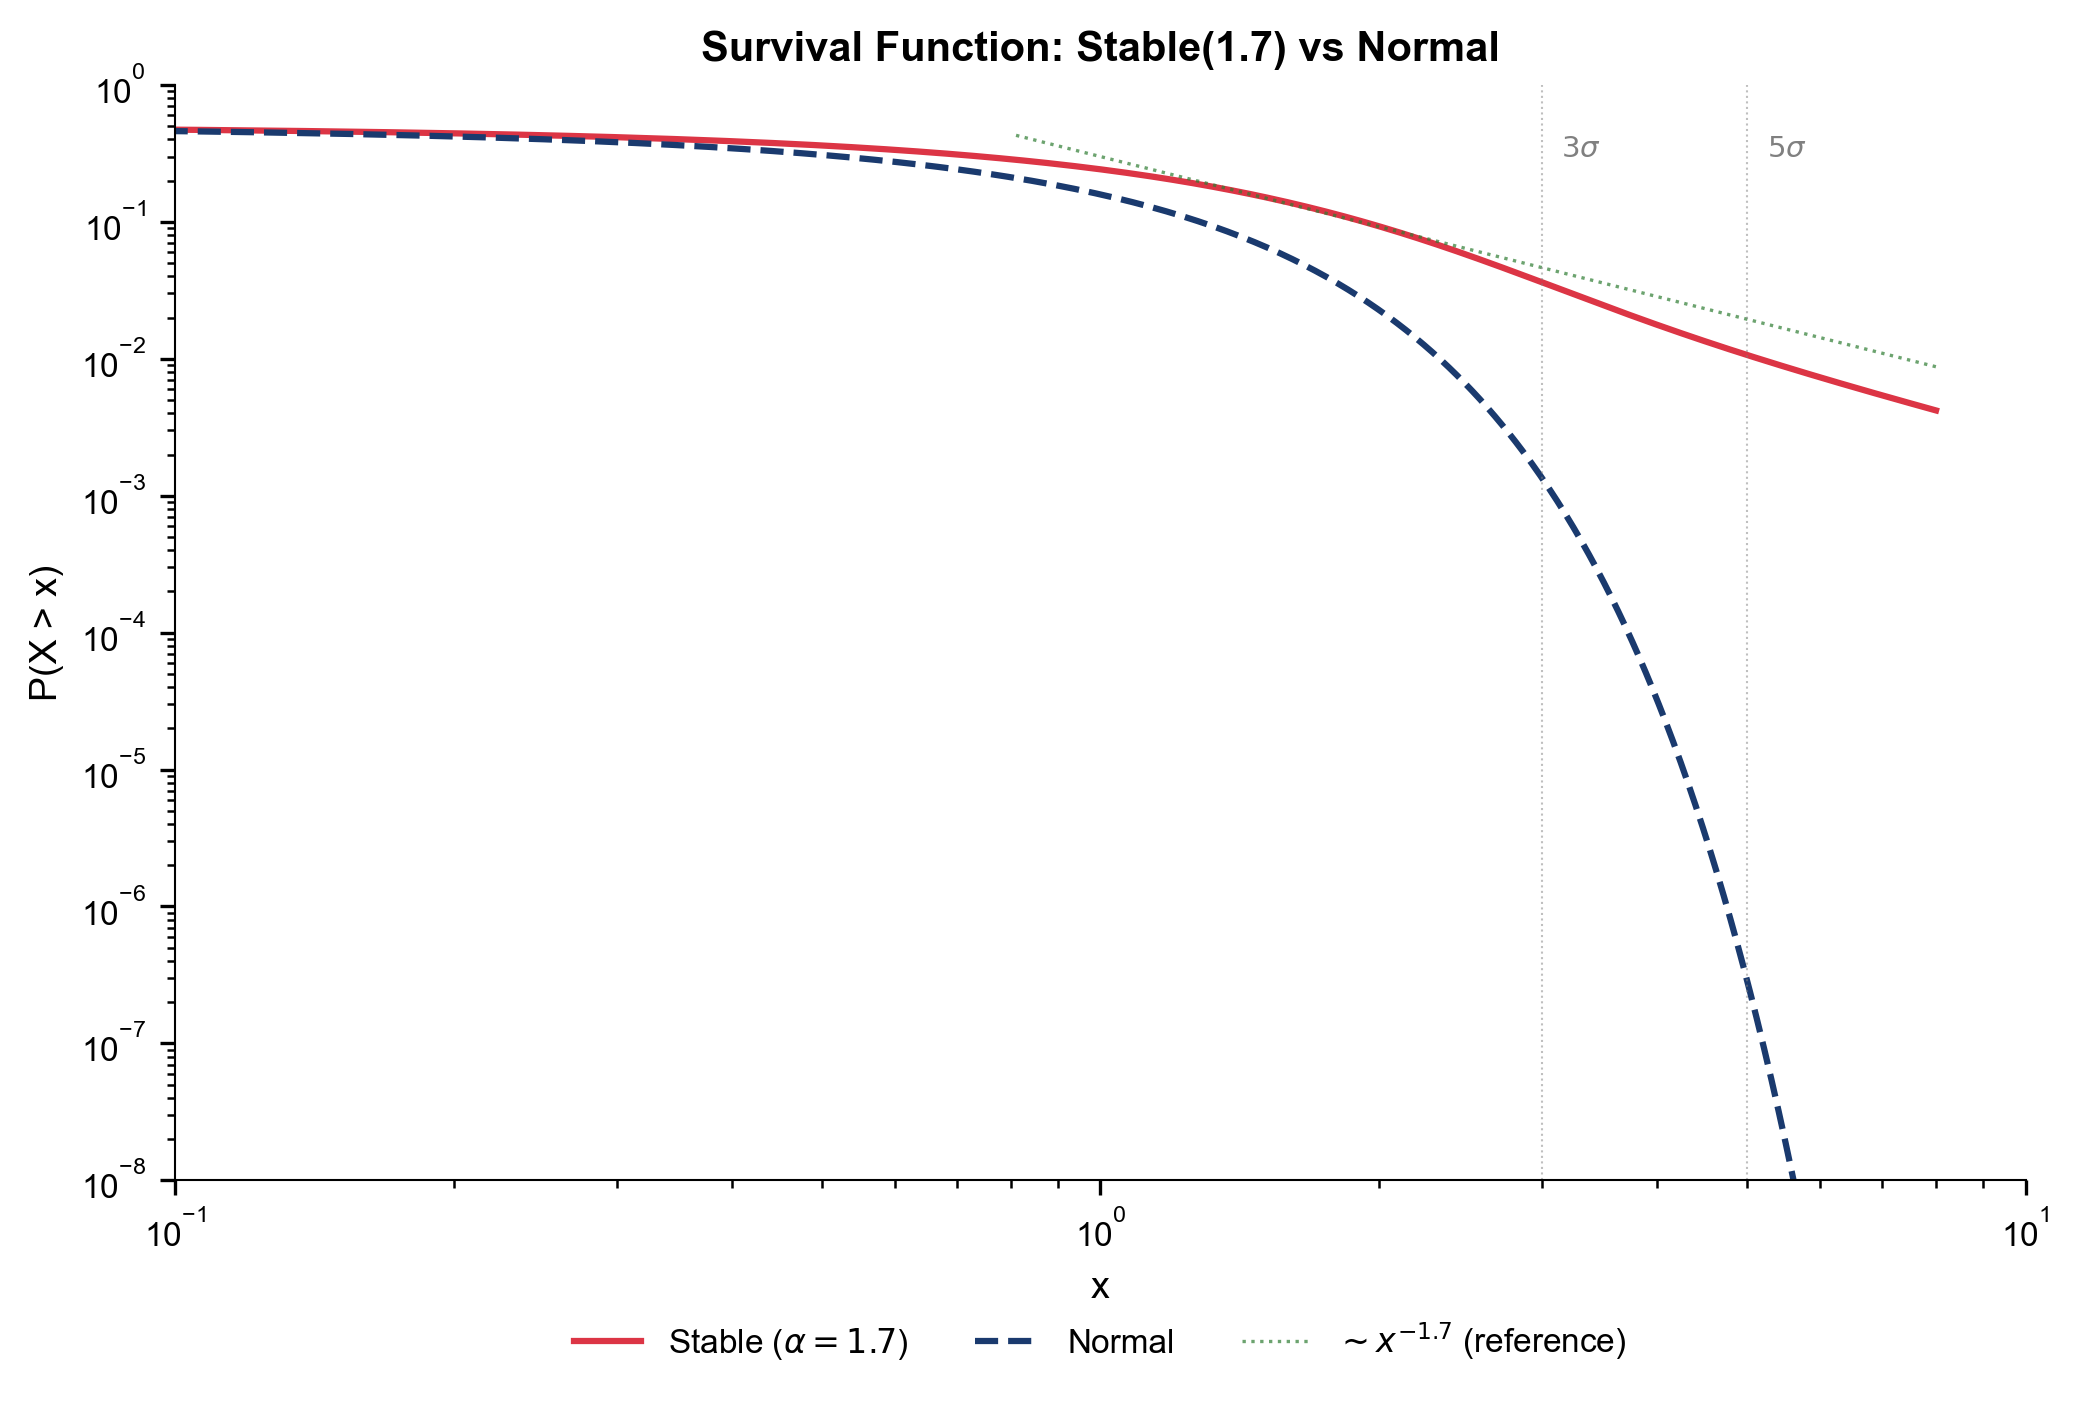
\includegraphics[width=0.25\textwidth]{ch2_tail_survival.png}
\end{center}
\quantlet{SFM\_ch2\_tail\_survival}{https://github.com/QuantLet/Stat_fin_markets/tree/master/Ch_02/SFM_ch2_stable_distributions}
\end{frame}

%--- Y3 Slide 13 ---
\slidelevel{Y3}
\begin{frame}{Exemplu: Interpretarea parametrilor stabili}
\begin{exampleblock}{Exercițiu: MLE pe S\&P~500 (2000--2023)}
$\hat{\alpha} = 1{,}70$, $\hat{\beta} = -0{,}10$, $\hat{\gamma} = 0{,}0058$, $\hat{\delta} = 0{,}0003$. Interpretați parametrii.
\end{exampleblock}

\begin{block}{Interpretare}
\begin{itemize}
\item $\hat{\alpha} = 1{,}70 < 2$: \textbf{varianță infinită} --- cozile descresc ca $|x|^{-1{,}70}$, mai lent decât $e^{-x^2/2}$
\item $\hat{\beta} = -0{,}10 < 0$: ușoară \textbf{asimetrie la stânga} --- coada pierdere mai grea
\item $\hat{\gamma} = 0{,}0058$: parametru de \textbf{scală} (analog $\sigma$, dar $\sigma^2 = \infty$)
\item $\hat{\delta} = 0{,}0003$: \textbf{locația} (randamentul mediu zilnic $\approx 0{,}03\%$)
\end{itemize}
\end{block}

\begin{alertblock}{Consecință}
\begin{itemize}
\item Dacă $\alpha = 1{,}70$, $P(|r| > 5\hat{\gamma})$ este de $\sim$12$\times$ mai mare decât sub distribuția normală
\item Markowitz medie-varianță \textbf{nu este validă}
\end{itemize}
\end{alertblock}
\end{frame}

%=============================================================================
% TITLU PARTEA II
%=============================================================================
% SECȚIUNEA 8: TEORIA VALORILOR EXTREME (EVT)
%=============================================================================
\section{Teoria Valorilor Extreme (EVT)}

%--- Y3 Slide 1 ---
\slidelevel{Y3}
\begin{frame}{EVT --- Motivație}
\begin{itemize}
\item Avem nevoie de modele precise pentru \textbf{evenimente extreme} (crize financiare, prăbușiri)
\item În loc să modelăm \textit{întreaga} distribuție, EVT se concentrează doar pe \textbf{cozi}
\item \textbf{Indicele de coadă $\xi$}: un singur număr care rezumă grosimea cozii
\begin{itemize}
\item $\xi > 0$: cozi groase (\textit{heavy tails}, descreștere tip lege putere) --- tipic pentru date financiare
\item $\xi = 0$: cozi exponențiale (similar cu distribuția normală)
\item $\xi < 0$: cozi mărginite (maximum finit)
\end{itemize}
\item Date financiare: $\hat{\xi} > 0$ confirmă că evenimentele extreme sunt mai frecvente decât prevede distribuția normală
\end{itemize}

\vspace{0.2cm}
\begin{block}{Idee cheie}
\begin{itemize}
\item EVT oferă \textbf{extrapolare riguroasă matematic} în cozi, chiar dincolo de datele observate
\end{itemize}
\end{block}
\end{frame}

%--- Y3 Slide 2 ---
\slidelevel{Y3}
\begin{frame}{GPD --- Introducere descriptivă}
\begin{itemize}
\item \textbf{Depășirile} peste un prag ridicat $u$ tind să urmeze o formă specifică:
\[
\text{Distribuția Pareto Generalizată (GPD)}
\]
\item Gândiți-vă astfel: ,,dat fiind că s-a întâmplat ceva extrem, cât de extrem a fost?''
\item GPD are doi parametri: formă $\xi$ și scală $\sigma$
\item Pentru date financiare, de regulă $\hat{\xi} \in [0{,}1;\ 0{,}5]$
\end{itemize}

\vspace{0.1cm}
\begin{center}
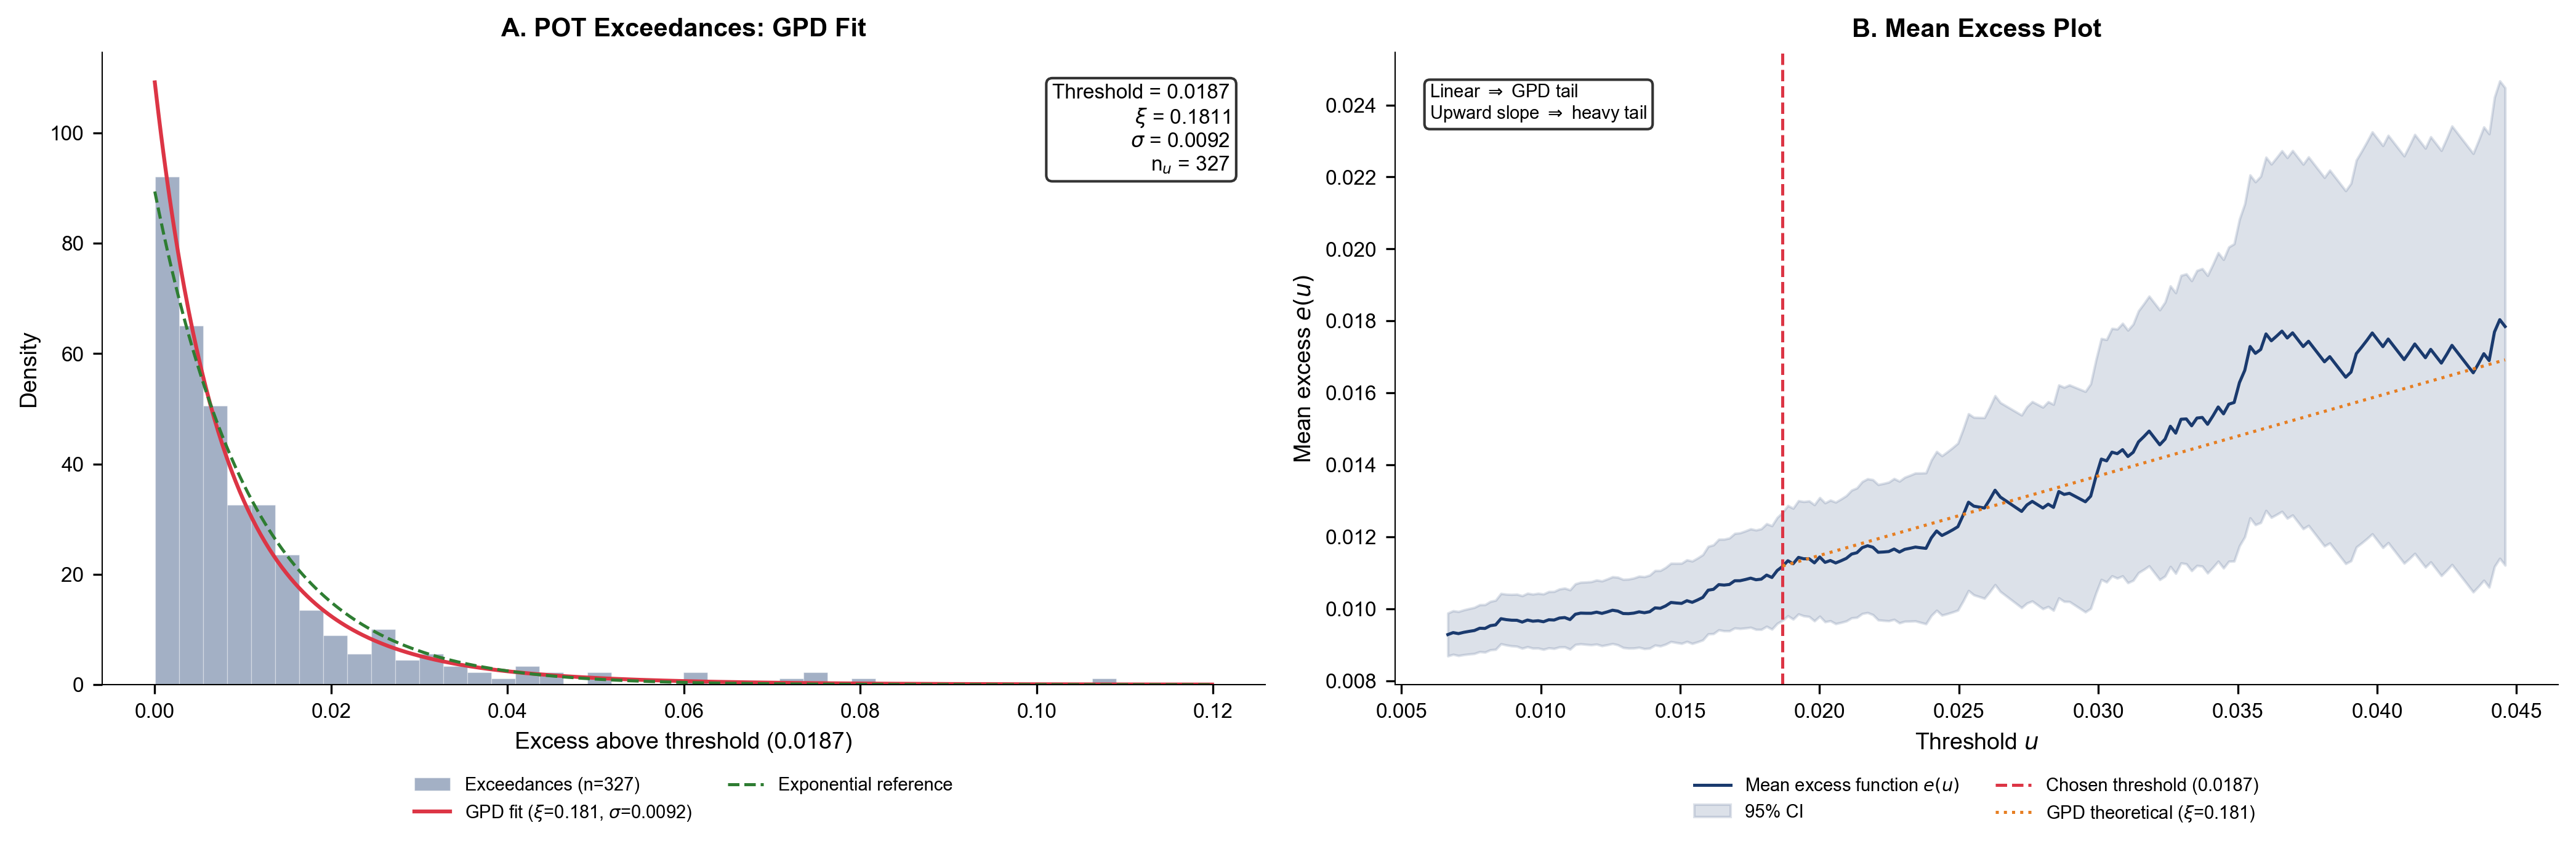
\includegraphics[width=0.42\textwidth]{ch2_evt_gpd_pot.png}
\end{center}
\quantlet{SFM\_ch2\_evt\_gpd}{https://github.com/QuantLet/Stat_fin_markets/tree/master/Ch_02/SFM_ch2_extreme_value}
\end{frame}

%--- Y3 Slide 3 ---
\slidelevel{Y3}
\begin{frame}{EVT în practică --- Evenimente extreme}
\begin{center}
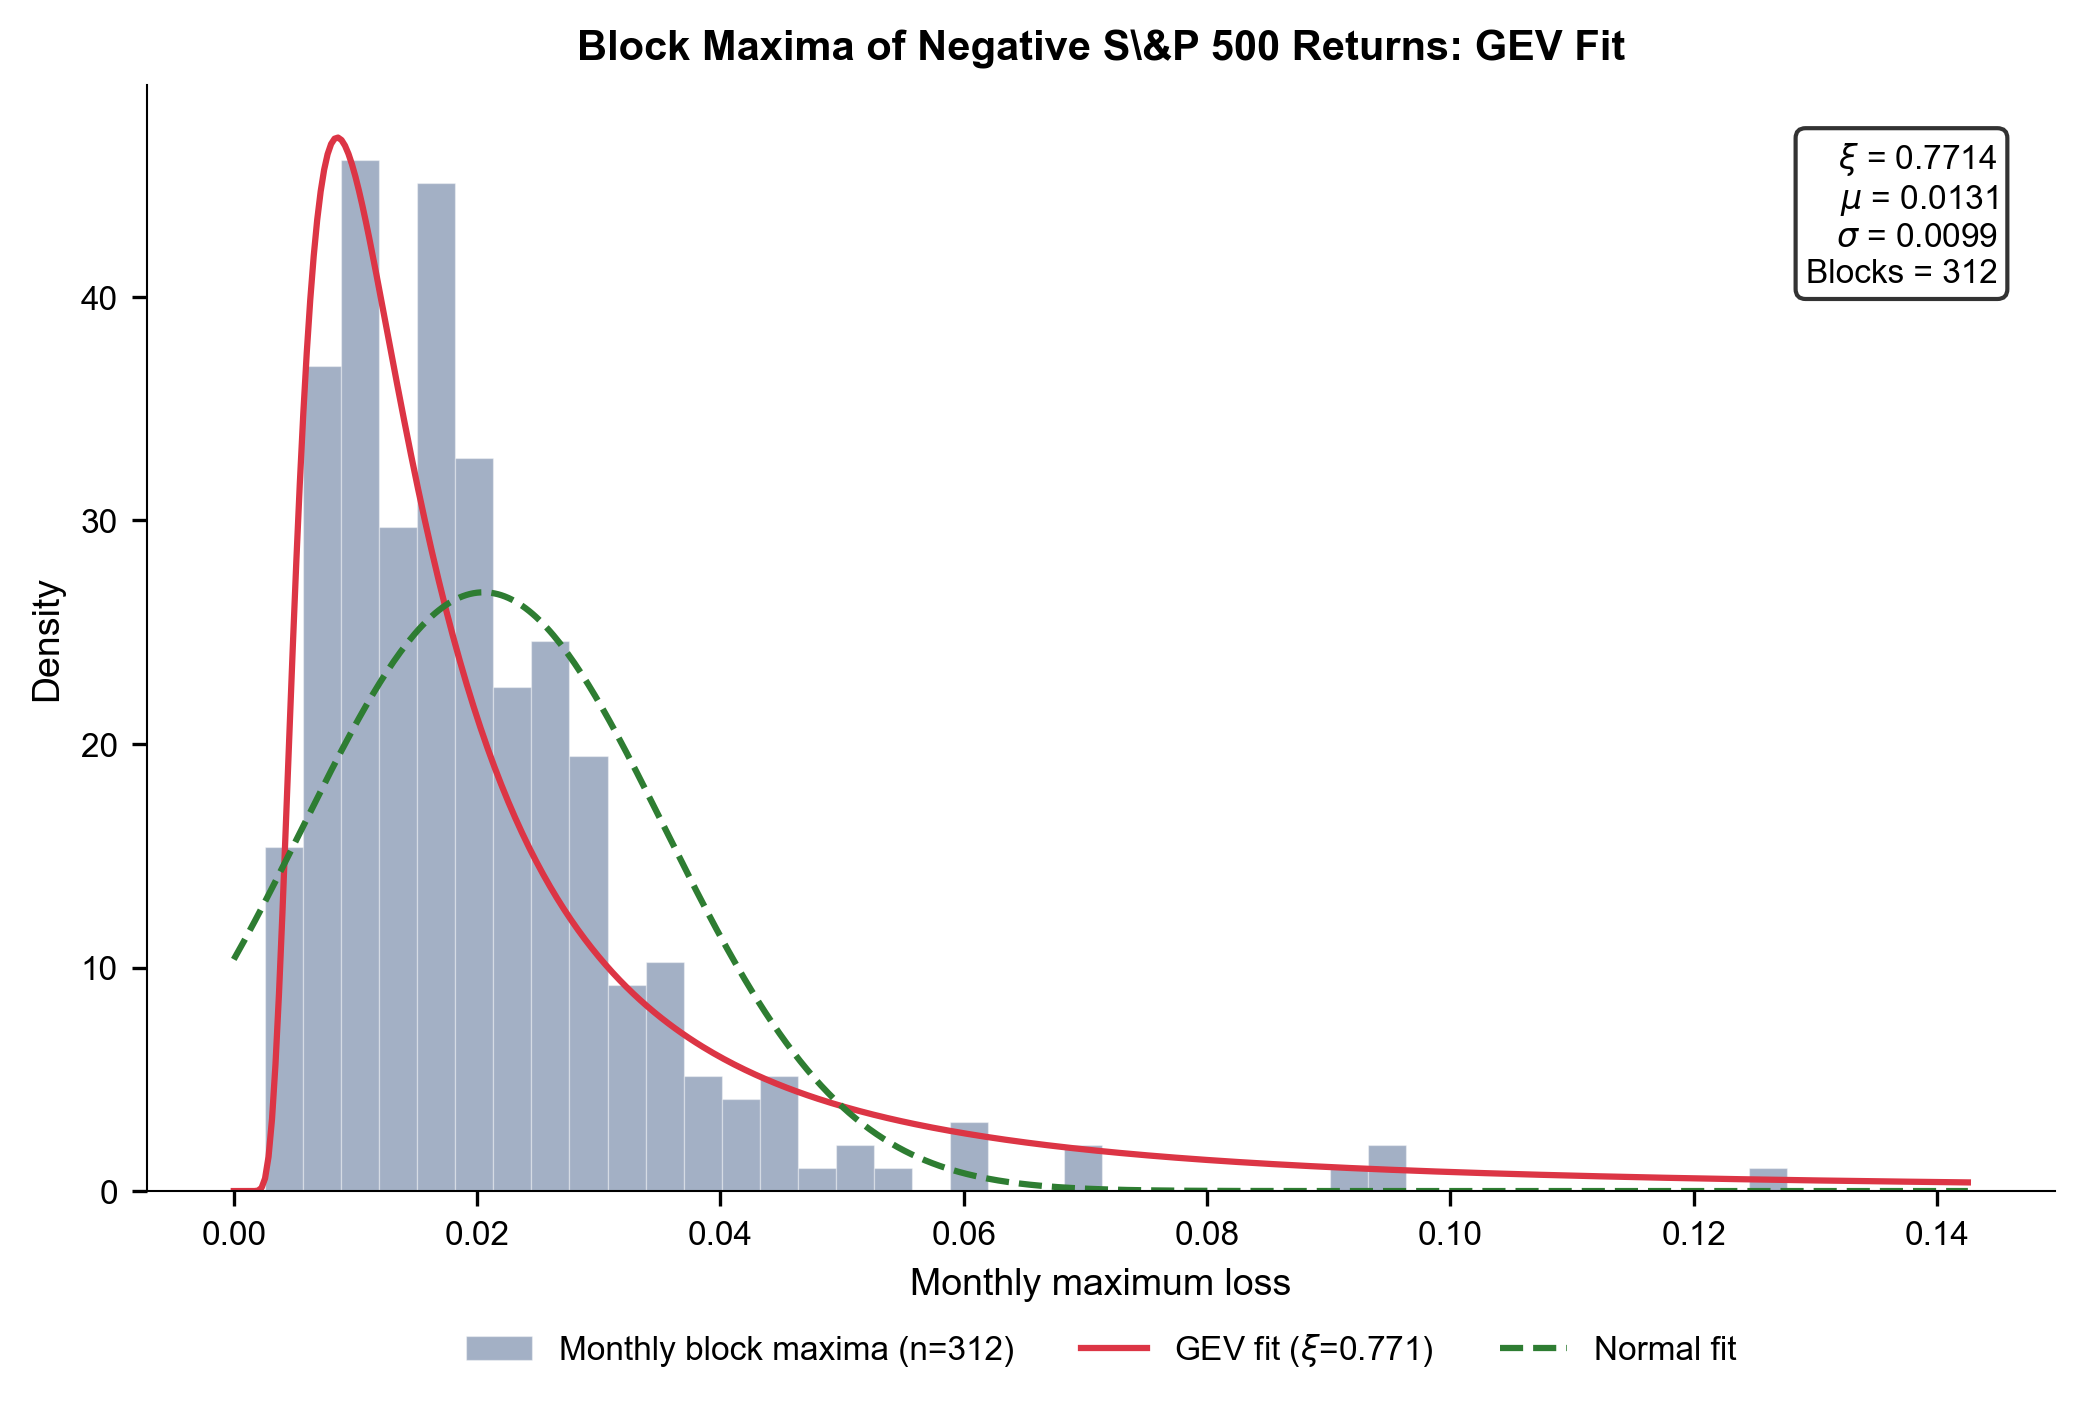
\includegraphics[width=0.45\textwidth]{ch2_evt_gev_fit.png}
\end{center}
\quantlet{SFM\_ch2\_evt\_gev}{https://github.com/QuantLet/Stat_fin_markets/tree/master/Ch_02/SFM_ch2_extreme_value}
\begin{itemize}
\item Maximele pe blocuri (ex.: cea mai mare pierdere lunară) urmează distribuția GEV
\item Teoreme formale la nivel Master; VaR/ES bazate pe EVT în secțiunea de managementul riscului
\end{itemize}
\end{frame}

%--- MSc Slide 4 ---
\slidelevel{MSc}
\begin{frame}{Teorema Fisher--Tippett--Gnedenko}
\begin{thm}[Fisher--Tippett--Gnedenko]
Dacă $M_n = \max(X_1, \ldots, X_n)$ și $\frac{M_n - b_n}{a_n} \xrightarrow{d} H$, atunci $H$ este \textbf{GEV}:
\[
H(x;\xi,\mu,\sigma) = \exp\!\left\{-\left(1 + \xi\frac{x-\mu}{\sigma}\right)^{-1/\xi}\right\}
\]
\end{thm}

\begin{itemize}
\item Trei tipuri în funcție de $\xi$:
\begin{itemize}
\item $\xi > 0$: \textbf{Fr\'{e}chet} --- cozi groase (date financiare)
\item $\xi = 0$: \textbf{Gumbel} --- cozi exponențiale
\item $\xi < 0$: \textbf{Weibull} --- cozi mărginite
\end{itemize}
\item Analog TLC dar pentru \textit{maxime} în loc de sume
\end{itemize}
\end{frame}

%--- MSc Slide 4b ---
\slidelevel{MSc}
\begin{frame}{Densitățile GEV --- Cele trei familii}
\begin{center}
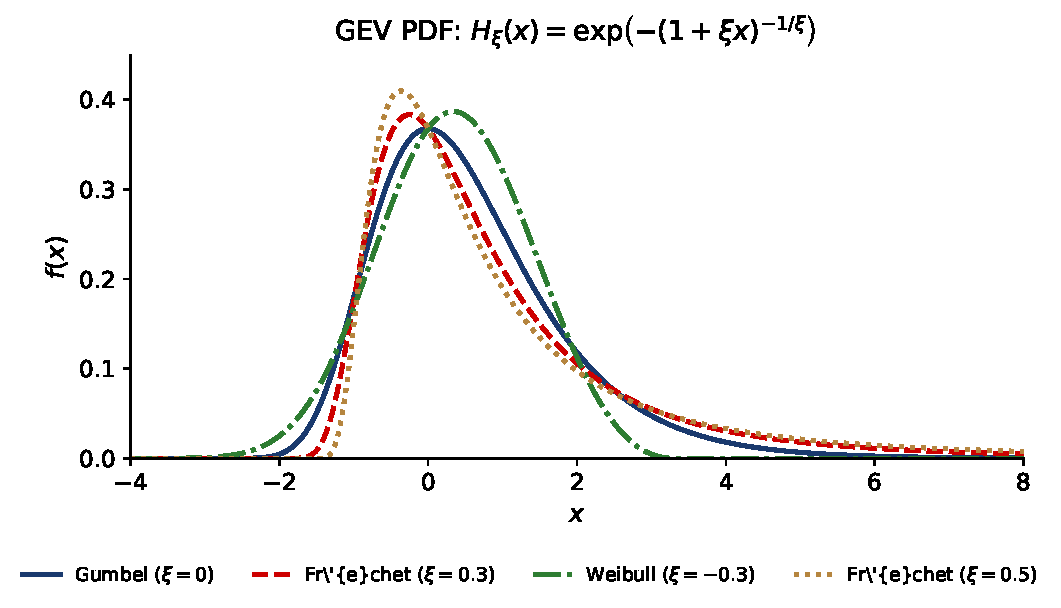
\includegraphics[width=0.58\textwidth]{ch2_gev_pdf_theoretical.pdf}
\end{center}
\begin{itemize}
\item \textbf{Fréchet} ($\xi > 0$): coadă dreaptă grea --- tipică pentru maxime financiare
\item \textbf{Gumbel} ($\xi = 0$): coadă exponențială
\item \textbf{Weibull} ($\xi < 0$): coadă mărginită (maximum finit)
\end{itemize}
\end{frame}

%--- MSc Slide 5 ---
\slidelevel{MSc}
\begin{frame}{Pickands--Balkema--de Haan și metoda POT}
\begin{thm}[Pickands--Balkema--de Haan]
Pentru un prag ridicat $u$, depășirile $Y = X - u \mid X > u$ urmează GPD:
\[
G(y;\xi,\sigma) = 1 - \left(1 + \xi\frac{y}{\sigma}\right)^{-1/\xi}, \quad y > 0.
\]
\end{thm}

\begin{itemize}
\item \textbf{Metoda POT} (Peaks Over Threshold):
\begin{enumerate}
\item Alegem pragul $u$ (graficul excesului mediu, stabilitatea parametrilor)
\item Ajustăm GPD pe depășiri prin MLE
\item Raportăm $(\hat{\xi}, \hat{\sigma})$
\end{enumerate}
\item \textbf{Funcția excesului mediu}: $e(u) = \E[X - u \mid X > u] = \frac{\sigma + \xi u}{1 - \xi}$
\item Liniară în $u$ pentru GPD $\Rightarrow$ instrument diagnostic pentru selectarea pragului
\end{itemize}
\end{frame}

%--- MSc Slide 5b ---
\slidelevel{MSc}
\begin{frame}{Densitățile GPD --- Forme în funcție de $\xi$}
\vspace{-0.2cm}
\begin{center}
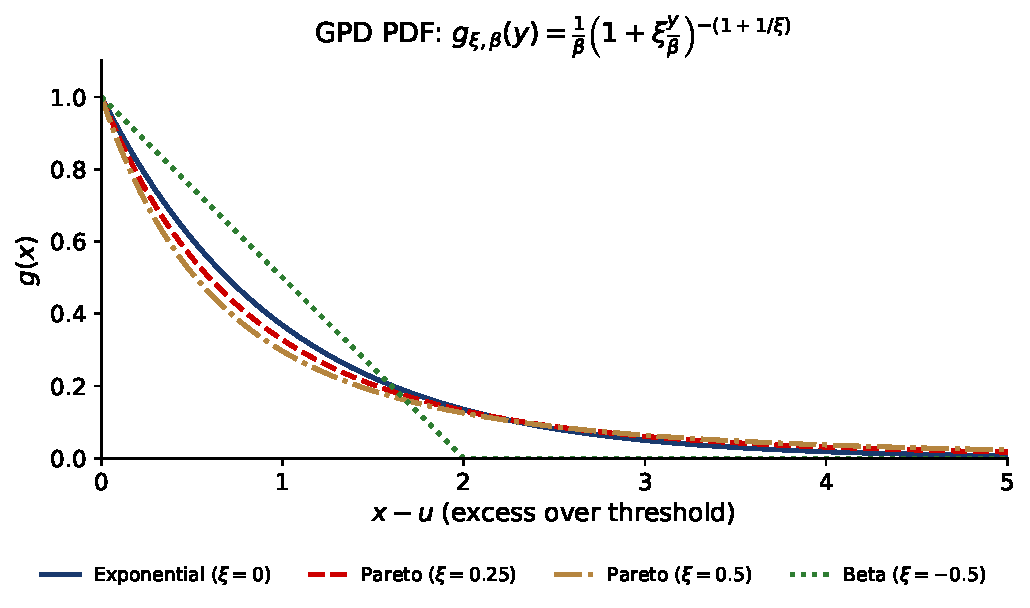
\includegraphics[width=0.52\textwidth]{ch2_gpd_pdf_theoretical.pdf}
\end{center}
\vspace{-0.2cm}
\begin{itemize}
\item $\xi > 0$ (\textbf{Pareto}): coadă grea --- tipică pentru depășiri financiare
\item $\xi = 0$ (\textbf{Exponențială}): referință; \quad $\xi < 0$ (\textbf{Beta}): suport finit
\item Cu cât $\xi$ este mai mare, cu atât depășirile extreme sunt \textbf{mai probabile}
\end{itemize}
\end{frame}

%--- MSc Slide 6 ---
\slidelevel{MSc}
\begin{frame}{VaR și ES bazate pe EVT}
\begin{itemize}
\item \textbf{VaR din GPD}:
\[
\text{VaR}_\alpha = u + \frac{\sigma}{\xi}\!\left[\left(\frac{n\alpha}{N_u}\right)^{-\xi} - 1\right]
\]
unde $N_u$ = numărul de depășiri, $n$ = observații totale
\item \textbf{ES din GPD}: $\text{ES}_\alpha = \frac{\text{VaR}_\alpha}{1-\xi} + \frac{\sigma - \xi u}{1-\xi}$, \quad $\xi < 1$
\end{itemize}

\vspace{0.2cm}
\begin{center}
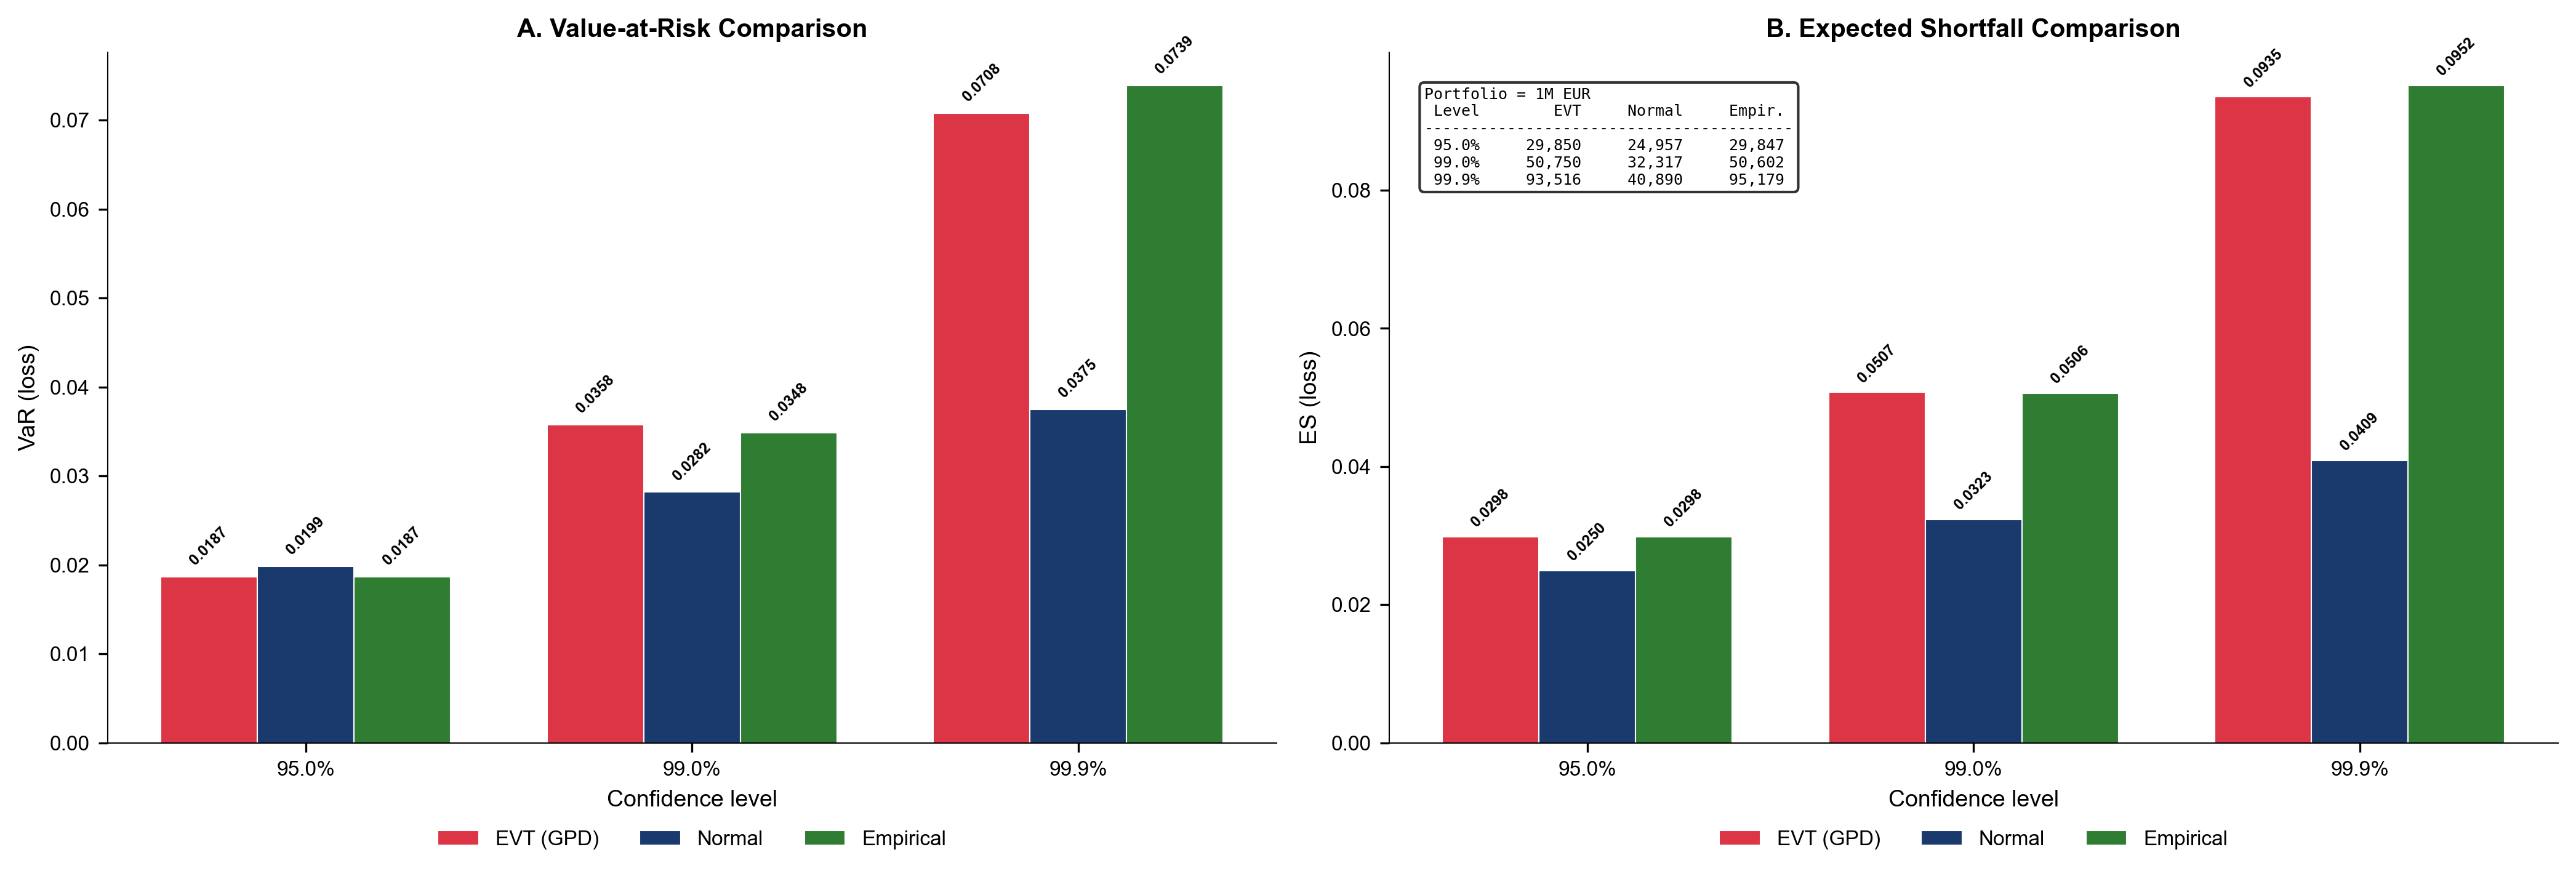
\includegraphics[width=0.6\textwidth]{ch2_evt_var_es.png}
\end{center}
\quantlet{SFM\_ch2\_evt\_var\_es}{https://github.com/QuantLet/Stat_fin_markets/tree/master/Ch_02/SFM_ch2_extreme_value}
\end{frame}

%--- MSc Slide 7 ---
\slidelevel{MSc}
\begin{frame}{Selectarea pragului}
\begin{itemize}
\item \textbf{Graficul excesului mediu}: $\hat{e}(u)$ vs.\ $u$; linearitatea sugerează că GPD este adecvată deasupra acelui $u$
\item \textbf{Graficul stabilității parametrilor}: $\hat{\xi}(u)$ și $\hat{\sigma}^*(u)$ vs.\ $u$; regiunea stabilă = prag bun
\item Compromis: $u$ prea mic $\Rightarrow$ eroare sistematică (date non-extreme incluse); $u$ prea mare $\Rightarrow$ varianță mare (puține depășiri)
\item Regulă practică: se folosesc primele 5--10\% din observații
\end{itemize}

\vspace{-0.1cm}
\begin{center}
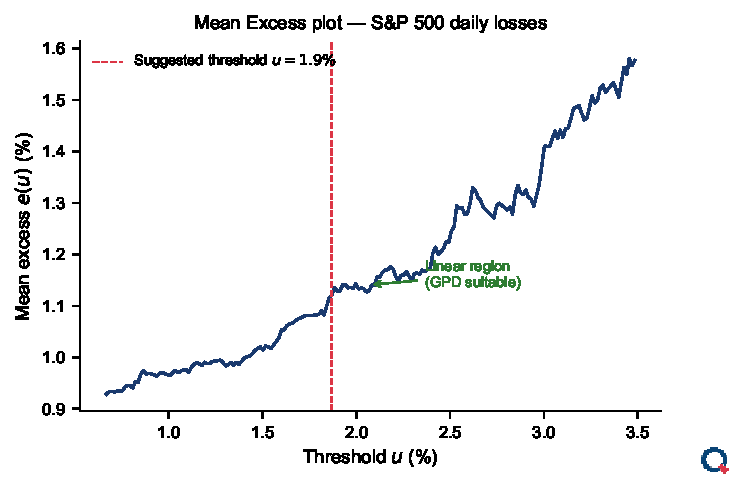
\includegraphics[width=0.4\textwidth]{ch2_mean_excess_plot.pdf}
\end{center}
\quantlet{SFM\_ch2\_mean\_excess}{https://github.com/QuantLet/Stat_fin_markets/tree/master/Ch_02/SFM_ch2_extreme_value}
\end{frame}

%--- PhD Slide 8 ---
\slidelevel{PhD}
\begin{frame}{Estimatorul Hill}
\begin{defn}[Estimatorul Hill]
Pentru statisticile de ordine (\textit{order statistics}) $X_{(1)} \geq X_{(2)} \geq \cdots \geq X_{(n)}$:
\[
\hat{\xi}_{\text{Hill}}^{(k)} = \frac{1}{k}\sum_{i=1}^{k}\ln X_{(i)} - \ln X_{(k+1)}, \quad k = 1, \ldots, n-1.
\]
Indicele de coadă este $\alpha = 1/\hat{\xi}_{\text{Hill}}$.
\end{defn}

\begin{itemize}
\item \textbf{Graficul Hill (\textit{Hill plot})}: $\hat{\xi}_{\text{Hill}}^{(k)}$ vs.\ $k$; regiunea stabilă indică $k$ adecvat
\item \textbf{Compromis bias-varianță}: $k$ mic $\Rightarrow$ varianță mare; $k$ mare $\Rightarrow$ eroare sistematică mare
\item Valid doar pentru $\xi > 0$ (cozi groase)
\end{itemize}
\end{frame}

%--- PhD Slide 9 ---
\slidelevel{PhD}
\begin{frame}{Estimatori alternativi ai indicelui de coadă}
\begin{itemize}
\item \textbf{Estimatorul Pickands}:
\[
\hat{\xi} = \frac{1}{\ln 2}\ln\frac{X_{(k)} - X_{(2k)}}{X_{(2k)} - X_{(4k)}}
\]
Funcționează pentru orice $\xi \in \R$ (nu doar $\xi > 0$)
\item \textbf{Estimatorul de momente} (Dekkers--Einmahl--de Haan): funcționează și el pentru orice $\xi$
\item \textbf{Condiții de ordin secund}: Hall (1982) --- parametrul de ordin secund $\rho$ guvernează $k$ optim în estimatorul Hill
\item \textbf{Selectare adaptivă a pragului}: minimizarea MSE asimptotică (Danielsson et al., 2001)
\end{itemize}
\end{frame}

%--- PhD Slide 9b ---
\slidelevel{PhD}
\begin{frame}{Graficul Hill --- S\&P 500}
\begin{center}
\includegraphics[width=0.7\textwidth]{ch2_hill_plot.pdf}
\end{center}
\quantlet{SFM\_ch2\_hill}{https://github.com/QuantLet/Stat_fin_markets/tree/master/Ch_02/SFM_ch2_extreme_value}
\vspace{-0.3cm}
\begin{itemize}
\item Stânga: $\hat{\alpha}_{\text{Hill}}^{(k)}$ vs.\ $k$ --- regiunea stabilă ($k \in [100, 300]$) sugerează $\hat{\alpha} \approx 3{,}5$
\item Dreapta: log-log confirmă legea putere (\textit{power law}); distribuția normală (punctată) curbează în jos
\end{itemize}
\end{frame}

%--- PhD Slide 10 ---
\slidelevel{PhD}
\begin{frame}{Conexiunea cu distribuțiile stabile}
\begin{itemize}
\item Dacă $X \sim S(\alpha, \beta, \gamma, \delta)$ cu $\alpha < 2$, atunci parametrul de formă EVT este:
\[
\xi = 1/\alpha
\]
\item Distribuțiile stabile sunt în domeniul de atracție al GEV Fr\'{e}chet ($\xi > 0$)
\item Estimatorul Hill aplicat pe date stabile: $\hat{\alpha}_{\text{Hill}} = 1/\hat{\xi}_{\text{Hill}}$
\item Compararea indicilor de coadă (\textit{tail indices}):
\begin{itemize}
\item Ajustare stabilă: $\hat{\alpha} \approx 1{,}7$ $\Rightarrow$ $\hat{\xi} \approx 0{,}59$
\item Estimarea Hill: dă de regulă $\hat{\alpha} \in [3, 5]$ (pentru cozi moderate)
\item Discrepanța apare deoarece Hill măsoară descreșterea \textit{locală} a cozii, iar $\alpha$ stabil guvernează forma \textit{globală}
\end{itemize}
\end{itemize}
\end{frame}

%--- Y3 Slide 11 ---
\slidelevel{Y3}
\begin{frame}{Exemplu POT --- VaR și ES pas cu pas}
\begin{exampleblock}{Exercițiu}
$n = 1{.}000$ randamente zilnice. Pragul $u = 2{,}5\%$ dă $N_u = 50$ depășiri. MLE pe depășiri: $\hat{\xi} = 0{,}3$, $\hat{\sigma} = 0{,}8\%$. Calculați $\text{VaR}_{1\%}$ și $\text{ES}_{1\%}$.
\end{exampleblock}

\begin{block}{Rezolvare}
\begin{enumerate}
\item Raportul: $\frac{n\alpha}{N_u} = \frac{1000 \times 0{,}01}{50} = 0{,}2$; \quad $0{,}2^{-0{,}3} = 1{,}621$
\item $\text{VaR}_{0{,}01} = u + \frac{\hat{\sigma}}{\hat{\xi}}[0{,}2^{-\hat{\xi}} - 1] = 2{,}5\% + 2{,}667\% \times 0{,}621 = \mathbf{4{,}16\%}$
\item $\text{ES}_{0{,}01} = \frac{\text{VaR}}{1-\hat{\xi}} + \frac{\hat{\sigma} - \hat{\xi}u}{1-\hat{\xi}} = \frac{4{,}16\%}{0{,}7} + \frac{0{,}05\%}{0{,}7} = \mathbf{6{,}01\%}$
\end{enumerate}
\end{block}

\begin{rmk}
\begin{itemize}
\item Comparație: VaR normală $= 3{,}49\%$, VaR EVT $= 4{,}16\%$ (\textbf{+19\%}); ES EVT $= 6{,}01\%$
\end{itemize}
\end{rmk}
\end{frame}

%=============================================================================
% ACTUALIZARE CUPRINS după Secțiunea 8
%=============================================================================
{
\setbeamertemplate{headline}{%
    \vskip10pt%
    \hbox to \paperwidth{\hskip0.5cm\hfill\hskip0.5cm}%
    \vskip4pt%
    {\color{FooterGray}\hrule height 0.4pt}%
}
\begin{frame}{}
    {\color{FooterGray}\hrule height 0.4pt}
    \vspace{0.1cm}
    {\Large\textcolor{IDAred}{\textbf{Cuprins}}}
    \vspace{0.2cm}
    {\small
    \begin{columns}[T]
        \begin{column}{0.48\textwidth}
            \begin{itemize}
                \item Introducere \checkmark
                \item De la prețuri la log-randamente \checkmark
                \item Distribuția normală \checkmark
                \item Fapte stilizate \checkmark
                \item Distribuția Student-$t$ \checkmark
                \item Distribuții asimetrice \checkmark
            \end{itemize}
        \end{column}
        \begin{column}{0.48\textwidth}
            \begin{itemize}
                \item Distribuții stabile \checkmark
                \item Teoria valorilor extreme \checkmark
                \item \textbf{Comparația distribuțiilor}
                \item Copule și dependența de coadă (\textit{tail dependence})
                \item Managementul riscului
                \item Extensii moderne / Rezumat
            \end{itemize}
        \end{column}
    \end{columns}
    }
\end{frame}
}

%=============================================================================
% SECȚIUNEA 9: COMPARAREA DISTRIBUȚIILOR ȘI SELECȚIA MODELULUI
%=============================================================================

%=============================================================================
% SECȚIUNEA 10: STUDIU DE CAZ
%=============================================================================
\section{Studiu de caz}

%--- Y3 Slide 1: Ajustări avansate ---
\slidelevel{Y3}
\begin{frame}{Studiu de caz: Ajustări avansate}
\quantlet{SFM\_ch2\_case\_study\_2b}{https://github.com/QuantLet/Stat_fin_markets/tree/master/Ch_02/SFM_ch2_case_study_2b}
    \begin{columns}[T]
        \begin{column}{0.55\textwidth}
            \begin{block}{Skew-t, Student-t, GED, Stabilă pe 3 piețe}
            \small
            Overlay pe histogramă (log-scale):
            \begin{itemize}\setlength{\itemsep}{0pt}
                \item \textcolor{MainBlue}{Student-t}: captează bine cozile, $\hat{\nu} \approx 3$--$5$
                \item \textcolor{Purple}{Skew-t} (Hansen): $\hat{\lambda} < 0$ surprinde asimetria stângă
                \item \textcolor{Forest}{GED}: $\hat{\nu} < 2$ confirmă leptokurtosis
                \item \textcolor{orange}{Stabilă}: $\hat{\alpha} < 2$ --- cozi cu lege de putere
            \end{itemize}
            \end{block}
        \end{column}
        \begin{column}{0.42\textwidth}
            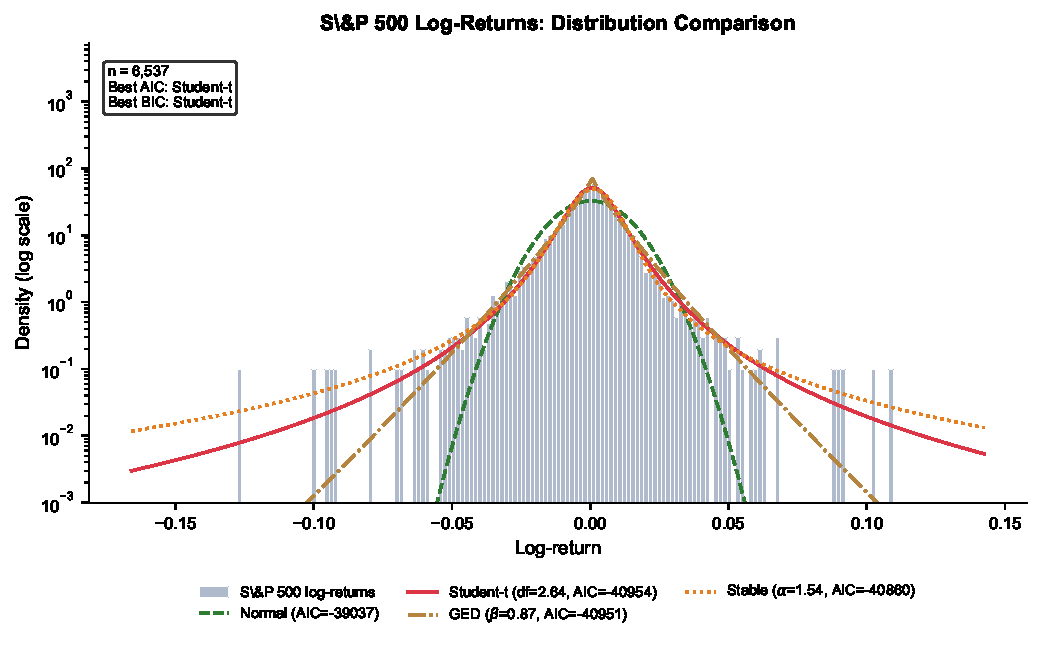
\includegraphics[width=\textwidth]{../../charts/ch2_dist_comparison_overlay.pdf}
        \end{column}
    \end{columns}
\end{frame}

%--- Y3 Slide 2: Parametrii estimați ---
\slidelevel{Y3}
\begin{frame}{Studiu de caz: Parametrii estimați}
    \begin{block}{Estimatori MLE pe cele 3 active (2015--2025)}
    \small
    {\centering
    \begin{tabular}{lccccc}
    \toprule
    \textbf{Activ} & \textbf{Student-t $\hat{\nu}$} & \textbf{Skew-t $\hat{\lambda}$} & \textbf{GED $\hat{\nu}$} & \textbf{Stabil $\hat{\alpha}$} & \textbf{Stabil $\hat{\beta}$} \\
    \midrule
    S\&P 500 & $4{,}5$ & $-0{,}15$ & $1{,}3$ & $1{,}75$ & $-0{,}15$ \\
    BRD      & $3{,}8$ & $-0{,}25$ & $1{,}2$ & $1{,}65$ & $-0{,}20$ \\
    Bitcoin  & $3{,}2$ & $-0{,}05$ & $1{,}1$ & $1{,}55$ & $-0{,}05$ \\
    \bottomrule
    \end{tabular}\par}
    \end{block}

    \begin{rmk}
    \begin{itemize}
    \item $\hat{\nu}_{t}$ scăzut $\Rightarrow$ cozi groase; $\hat{\alpha} < 2$ $\Rightarrow$ varianță posibil infinită; $\hat{\nu}_{\text{GED}} < 2$ $\Rightarrow$ cozi mai groase ca distribuția normală
    \item $\hat{\lambda} < 0$ (skew-t) și $\hat{\beta} < 0$ (stabil) $\Rightarrow$ asimetrie negativă (risc mai mare pe scăderi)
    \item Parametrii se estimează prin MLE; notație: $\nu$ este parametrul de formă atât pentru Student-$t$ cât și pentru GED
    \end{itemize}
    \end{rmk}
\end{frame}

%--- Y3 Slide 3: Comportamentul cozilor ---
\slidelevel{Y3}
\begin{frame}{Studiu de caz: Comportamentul cozilor}
\quantlet{SFM\_ch2\_case\_study\_2b}{https://github.com/QuantLet/Stat_fin_markets/tree/master/Ch_02/SFM_ch2_case_study_2b}
    \begin{columns}[T]
        \begin{column}{0.55\textwidth}
            \begin{block}{Grafic log-log survival}
            \small
            Funcția de supraviețuire $P(\text{Loss} > x)$ în coordonate log-log:
            \begin{itemize}\setlength{\itemsep}{0pt}
                \item Linie dreaptă $\Rightarrow$ \textbf{lege de putere}: $P(X > x) \sim x^{-\alpha}$
                \item \textcolor{Amber}{Normal}: cade prea rapid; \textcolor{IDAred}{Student-t}: urmărește mai bine datele
                \item Bitcoin: cozile cele mai groase, panta cea mai mică
            \end{itemize}
            \end{block}
        \end{column}
        \begin{column}{0.42\textwidth}
            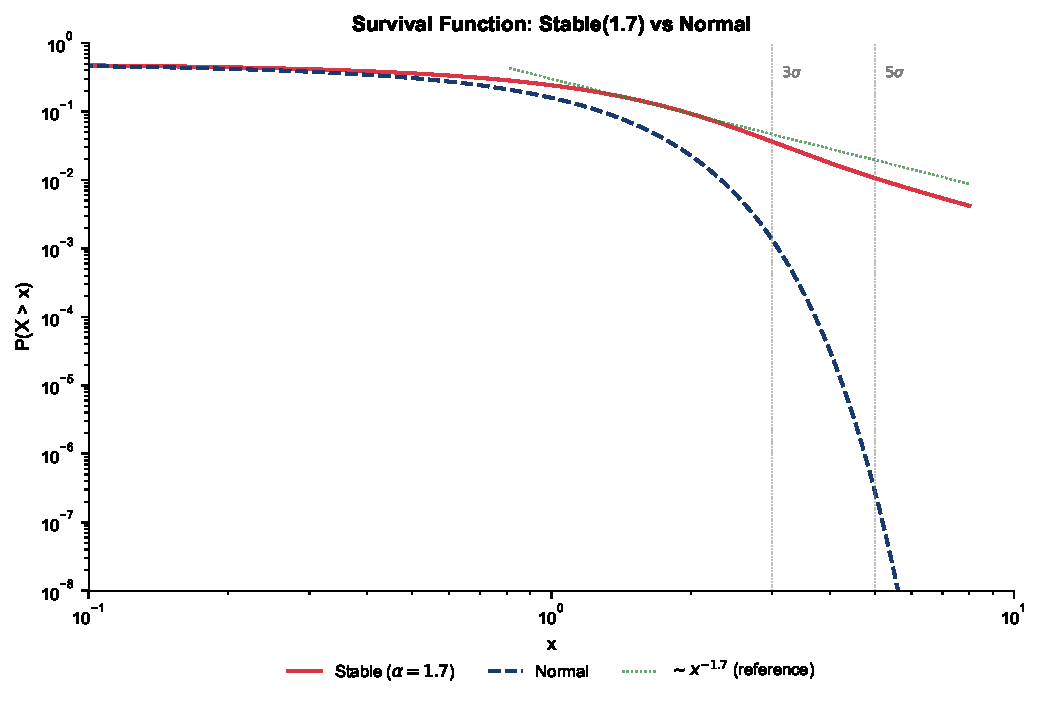
\includegraphics[width=\textwidth]{../../charts/ch2_tail_survival.pdf}
        \end{column}
    \end{columns}

\end{frame}

%--- Y3 Slide 4: Estimatorul Hill ---
\slidelevel{Y3}
\begin{frame}{Studiu de caz: Estimatorul Hill}
    \begin{columns}[T]
        \begin{column}{0.55\textwidth}
            \begin{block}{$\hat{\alpha}_{\text{Hill}}$ pe 3 piețe}
            \small
            \begin{itemize}\setlength{\itemsep}{0pt}
                \item S\&P 500: $\hat{\alpha} \approx 3$--$4$; \; BRD: $\approx 2{,}5$--$3{,}5$; \; Bitcoin: $\approx 2$--$3$
                \item Stabilitatea pe un platou validează estimarea
            \end{itemize}
            \end{block}
        \end{column}
        \begin{column}{0.42\textwidth}
            \includegraphics[width=\textwidth]{../../charts/ch2_hill_plot.pdf}
        \end{column}
    \end{columns}
    \vspace{-0.2cm}
    {\scriptsize $\hat{\alpha}_{\text{Hill}} < 2$ $\Rightarrow$ varianța \textbf{nu converge}. \; $\hat{\alpha}_{\text{Hill}} \approx 3$--$4$ vs.\ $\hat{\alpha}_{\text{stabil}} \approx 1{,}7$: Hill estimează \emph{local} coada, stabilă pe \emph{întreaga} distribuție.}
\end{frame}

%--- Y3 Slide 5: VaR/ES sub EVT ---
\slidelevel{Y3}
\begin{frame}{Studiu de caz: VaR/ES sub EVT}
\quantlet{SFM\_ch2\_case\_study\_2b}{https://github.com/QuantLet/Stat_fin_markets/tree/master/Ch_02/SFM_ch2_case_study_2b}
    \begin{columns}[T]
        \begin{column}{0.55\textwidth}
            \begin{block}{VaR/ES 1\%, 1M EUR, S\&P 500}
            \scriptsize
            GPD: $u\!=\!2{,}5\%$, $\hat{\xi}\!=\!0{,}28$, $\hat{\sigma}\!=\!0{,}8\%$, $N_u/n\!=\!5\%$
            \begin{itemize}\setlength{\itemsep}{0pt}
                \item \textcolor{MainBlue}{Normal}: VaR $26\,750$; ES $30\,500$
                \item \textcolor{IDAred}{Student-t} ($\hat{\nu}\!=\!4{,}5$): VaR $30\,400$; ES $40\,200$
                \item \textcolor{Purple}{Skew-t} ($\hat{\lambda}\!=\!-0{,}15$): VaR $33\,800$
                \item \textcolor{Forest}{EVT-GPD}: VaR $35\,200$; ES $50\,300$
            \end{itemize}
            \end{block}
        \end{column}
        \begin{column}{0.42\textwidth}
            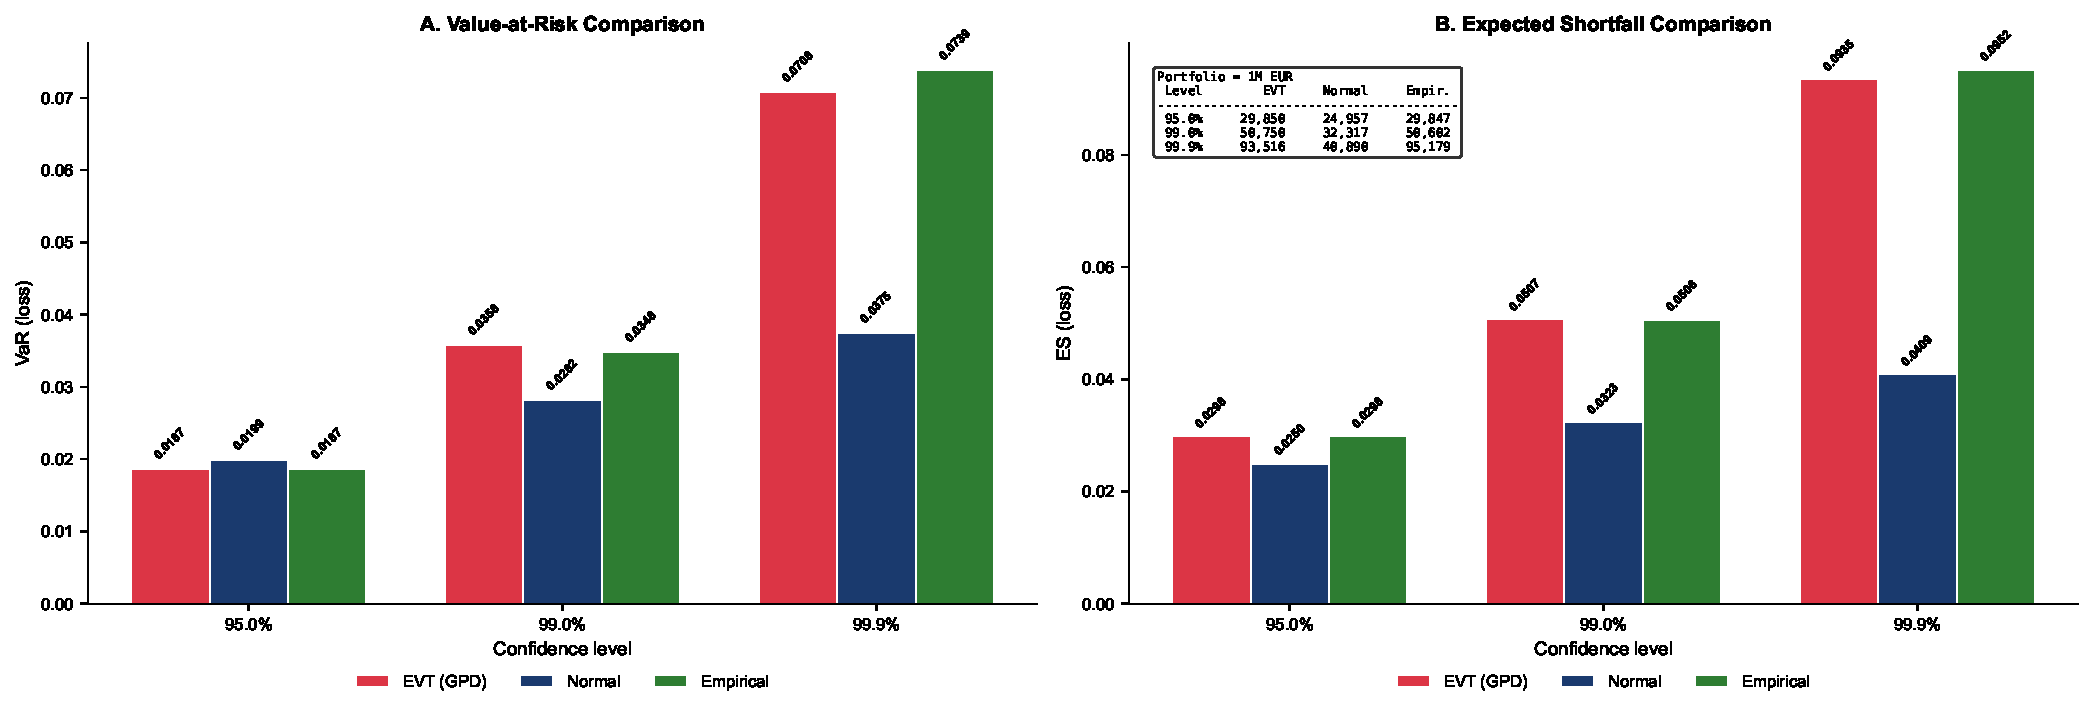
\includegraphics[width=\textwidth]{../../charts/ch2_evt_var_es.pdf}
        \end{column}
    \end{columns}
    \vspace{-0.3cm}
    {\tiny EVT: $\text{VaR}_{1\%}\!=\!u + \tfrac{\hat{\sigma}}{\hat{\xi}}\bigl[(\tfrac{n\alpha}{N_u})^{-\hat{\xi}}\!\!- 1\bigr]$; \; Skew-t: $+$15\% VaR vs.\ simetrică}
\end{frame}

%--- Y3 Slide 6: Concluzii ---
\slidelevel{Y3}
\begin{frame}{Studiu de caz: Concluzii}
    \begin{block}{Ierarhia modelelor (AIC $= -2\ell + 2k$; $\Delta\text{AIC} > 10$ vs.\ Normal)}
    \small
    \begin{enumerate}\setlength{\itemsep}{0pt}
        \item \textbf{Skew-t / GED / Student-t} --- cel mai bun compromis, date zilnice
        \item \textbf{Stabilă} --- utilă teoretic, estimare lentă
        \item \textbf{EVT-GPD} --- cea mai bună pentru cuantile extreme ($< 1\%$)
        \item \textbf{Normal} --- inadecvată, rămâne referință
    \end{enumerate}
    \end{block}

    \begin{alertblock}{Lecția principală}
        Nu există model universal: alegerea depinde de cuantilă (5\% vs 0.1\%), activ (acțiuni vs cripto), orizont (zilnic vs lunar).
    \end{alertblock}

    \begin{rmk}
    \begin{itemize}
    \item \textbf{Capitolul 4} formalizează selecția modelului și backtesting-ul
    \end{itemize}
    \end{rmk}
\end{frame}

%=============================================================================
% SECTIUNEA: QUIZ
%=============================================================================
\section{Quiz}
\slidelevel{Y3}
\begin{frame}{Întrebarea 3}
    \begin{cminipage}{0.95\textwidth}
    \begin{alertblock}{Întrebare}
        \begin{itemize}
            \item Care proprietate face distribuțiile $\alpha$-stabile unice din punct de vedere teoretic?
        \end{itemize}
    \end{alertblock}

    \vspace{0.3cm}

    \begin{block}{Variante de răspuns}

        \textcolor{MainBlue}{\textbf{(A)}} Au cozi exponențiale (scad rapid)\\[3pt]

        \textcolor{MainBlue}{\textbf{(B)}} Sunt singurele limite posibile ale sumelor normalizate (TLCG)\\[3pt]

        \textcolor{MainBlue}{\textbf{(C)}} Au întotdeauna varianță finită\\[3pt]

        \textcolor{MainBlue}{\textbf{(D)}} Sunt întotdeauna simetrice

    \end{block}
    \end{cminipage}
\end{frame}

\slidelevel{Y3}
\begin{frame}{Întrebarea 3: Răspuns}
    \begin{cminipage}{0.95\textwidth}
    \begin{exampleblock}{Răspuns: (B)}
    \begin{itemize}
        \item Teorema Limită Centrală Generalizată (TLCG) arată că distribuțiile stabile sunt \textbf{singurele} limite posibile ale sumelor normalizate de v.a.\ i.i.d.
        \item (A) este invers: distribuțiile stabile cu $\alpha < 2$ au cozi \textbf{groase} (lege putere), nu exponențiale.
        \item (C) este greșit: pentru $\alpha < 2$, varianța este infinită.
        \item (D) este greșit: parametrul $\beta \in [-1,1]$ controlează asimetria.
    \end{itemize}
    \end{exampleblock}
    \end{cminipage}
\end{frame}

\slidelevel{Y3}
\begin{frame}{Întrebarea 5}
    \begin{cminipage}{0.95\textwidth}
    \begin{alertblock}{Întrebare}
        \begin{itemize}
            \item În metoda Peaks-Over-Threshold (POT), ce distribuție se ajustează pe excesele peste prag (\textit{threshold exceedances})?
        \end{itemize}
    \end{alertblock}

    \vspace{0.3cm}

    \begin{block}{Variante de răspuns}

        \textcolor{MainBlue}{\textbf{(A)}} Distribuția normală\\[3pt]

        \textcolor{MainBlue}{\textbf{(B)}} Distribuția Pareto generalizată (GPD)\\[3pt]

        \textcolor{MainBlue}{\textbf{(C)}} Distribuția exponențială\\[3pt]

        \textcolor{MainBlue}{\textbf{(D)}} Distribuția GEV (Generalized Extreme Value)

    \end{block}
    \end{cminipage}
\end{frame}

\slidelevel{Y3}
\begin{frame}{Întrebarea 5: Răspuns}
    \begin{cminipage}{0.95\textwidth}
    \begin{exampleblock}{Răspuns: (B)}
    \begin{itemize}
        \item Teorema Pickands--Balkema--de Haan arată că excesele peste un prag $u$ suficient de mare converg la GPD.
        \item (A) este inadecvată: distribuția normală nu modelează cozile extreme.
        \item (C) este un caz particular: GPD cu $\xi = 0$ este exponențială, dar este prea restrictivă.
        \item (D) este pentru metoda Block Maxima, nu POT. GEV se ajustează pe maximele pe blocuri.
    \end{itemize}
    \end{exampleblock}
    \end{cminipage}
\end{frame}

%=============================================================================
% SECTIUNEA: EXERCITII DE EXAMEN
%=============================================================================
\section{Exercitii de examen}
\slidelevel{MSc}
\begin{frame}{Exercițiul 4: Distribuții stabile}
\begin{block}{Enunț}
Un cercetător ajustează o distribuție stabilă pe randamentele Bitcoin și obține $(\hat{\alpha}, \hat{\beta}, \hat{\gamma}, \hat{\delta}) = (1{,}72;\; -0{,}15;\; 0{,}008;\; 0{,}001)$.
\end{block}
\begin{enumerate}
    \item Interpretați fiecare parametru economic: ce spun $\alpha$, $\beta$, $\gamma$, $\delta$?
    \item Această distribuție are varianță finită? Justificați.
    \item Cum se compară cozile cu cele ale distribuției normale?
    \item Ce implică $\beta = -0{,}15$ pentru asimetria riscului?
\end{enumerate}
\vspace{0.1cm}
\begin{exampleblock}{De reținut}
$\alpha \in (0,2]$: indice de stabilitate (greutatea cozilor); $\beta \in [-1,1]$: asimetrie; $\gamma > 0$: scală; $\delta$: locație. Varianța finită doar dacă $\alpha = 2$.
\end{exampleblock}
\end{frame}

\slidelevel{MSc}
\begin{frame}{Exercițiul 5: EVT --- Metoda POT}
\begin{block}{Enunț}
Dintr-un eșantion de 2000 de randamente zilnice, 80 depășesc pragul $u = 3\%$ în valoare absolută. GPD ajustată: $\hat{\xi} = 0{,}25$, $\hat{\sigma} = 1{,}0\%$.
\end{block}
\begin{enumerate}
    \item Calculați VaR la nivelul 1\% folosind formula POT:
    \[
    \text{VaR}_\alpha = u + \frac{\hat{\sigma}}{\hat{\xi}}\left[\left(\frac{n}{N_u} \cdot \alpha\right)^{-\hat{\xi}} - 1\right]
    \]
    \item Calculați Expected Shortfall:
    $\text{ES}_\alpha = \frac{\text{VaR}_\alpha}{1-\hat{\xi}} + \frac{\hat{\sigma} - \hat{\xi}\cdot u}{1-\hat{\xi}}$
    \item Ce semnifică $\hat{\xi} > 0$? Ce clasă de distribuții implică?
    \item Cum influențează alegerea pragului $u$ calitatea estimării?
\end{enumerate}
\end{frame}

%=============================================================================
% LABORATOR PYTHON
%=============================================================================

\slidelevel{MSc}
\begin{frame}{Laborator Python --- Exerciții interactive}
\small
\begin{exampleblock}{Lab 2: Distribuții stabile (MSc)}
Rulați \texttt{SFM\_ch2\_stable\_distributions.ipynb}:
\begin{enumerate}
\item Estimați $(\hat{\alpha}, \hat{\beta}, \hat{\gamma}, \hat{\delta})$; grafic PDF stabilă vs.\ normală vs.\ Student-$t$
\item Calculați VaR 1\% sub toate cele trei modele. Raportați diferențele
\end{enumerate}
\end{exampleblock}
\quantlet{SFM\_ch2\_stable\_distributions}{https://github.com/QuantLet/Stat_fin_markets/tree/master/Ch_02/SFM_ch2_stable_distributions}
\begin{block}{Lab 3: EVT și backtesting (MSc)}
Folosind \texttt{SFM\_ch2\_extreme\_value.ipynb}:
\begin{enumerate}
\item Grafic Mean Excess; selectați prag $u$; ajustați GPD $\Rightarrow$ $(\hat{\xi}, \hat{\sigma})$
\item Calculați VaR 1\% și ES 1\% bazate pe EVT
\item Backtest VaR cu fereastră mobilă (\textit{rolling window}) de 250 zile; testul Kupiec
\end{enumerate}
\end{block}
\quantlet{SFM\_ch2\_extreme\_value}{https://github.com/QuantLet/Stat_fin_markets/tree/master/Ch_02/SFM_ch2_extreme_value}
\end{frame}

%=============================================================================
% REZOLVARI EXERCITII
%=============================================================================
\section*{Rezolvări exerciții}
\slidelevel{MSc}
\begin{frame}{Exercițiul 4: Rezolvare}
\begin{block}{Rezolvare}
Date: $(\hat{\alpha}, \hat{\beta}, \hat{\gamma}, \hat{\delta}) = (1{,}72,\; -0{,}15,\; 0{,}008,\; 0{,}001)$.

\textbf{1.} Interpretare:
\begin{itemize}
\item $\alpha = 1{,}72$: cozi groase (mai groase decât distribuția normală, $\alpha = 2$); mai aproape de Cauchy ($\alpha=1$)
\item $\beta = -0{,}15$: asimetrie negativă (\textit{negative skewness}) (coada stângă mai grea $\Rightarrow$ pierderi extreme mai probabile)
\item $\gamma = 0{,}008$: parametru de scală (similar deviației standard)
\item $\delta = 0{,}001$: locație (aproape de zero, randament mediu zilnic)
\end{itemize}

\textbf{2.} $\alpha = 1{,}72 < 2$ $\Rightarrow$ varianță \textbf{infinită}. Doar momentele de ordin $p < 1{,}72$ sunt finite.

\textbf{3.} Cozile scad ca $|x|^{-1{,}72-1} = |x|^{-2{,}72}$ vs.\ $e^{-x^2/2}$ (normală). Mult mai lent $\Rightarrow$ evenimente extreme mult mai probabile.

\textbf{4.} $\beta < 0$: coada stângă este mai grea decât coada dreaptă $\Rightarrow$ riscul de pierdere este asimetric.
\end{block}
\end{frame}

\slidelevel{MSc}
\begin{frame}{Exercițiul 5: Rezolvare}
\begin{block}{Rezolvare}
Date: $n = 2000$, $N_u = 80$, $u = 0{,}03$, $\hat{\xi} = 0{,}25$, $\hat{\sigma} = 0{,}01$, $\alpha = 0{,}01$.

\textbf{1.} VaR POT:
\[
\text{VaR}_{0{,}01} = 0{,}03 + \frac{0{,}01}{0{,}25}\left[\left(\frac{2000}{80}\cdot 0{,}01\right)^{-0{,}25} - 1\right] = 0{,}03 + 0{,}04\left[0{,}25^{-0{,}25} - 1\right]
\]
$0{,}25^{-0{,}25} = e^{0{,}25 \times 1{,}3863} = e^{0{,}3466} = 1{,}4142$; \;VaR $= 0{,}03 + 0{,}04 \times 0{,}4142 = 0{,}0466 = 4{,}66\%$

\textbf{2.} ES: $\text{ES}_{0{,}01} = \frac{0{,}0466}{1-0{,}25} + \frac{0{,}01 - 0{,}25 \times 0{,}03}{1-0{,}25} = 0{,}0621 + 0{,}0033 = 6{,}54\%$

\textbf{3.} $\hat{\xi} > 0$ $\Rightarrow$ domeniul Fréchet: cozi tip lege putere (cozi groase). Distribuția GPD are suport infinit.

\textbf{4.} Prag prea jos: bias (multe date non-extreme); prag prea sus: varianță mare (puține date). Se alege $u$ prin graficul Mean Excess.
\end{block}
\end{frame}

%=============================================================================
% ANEXĂ: APROFUNDARE --- DISTRIBUȚII STABILE (PhD)
%=============================================================================

\section*{Anexă: Aprofundare --- Distribuții stabile}

%--- PhD Slide A1 (fost Slide 9b) ---
\slidelevel{PhD}
\begin{frame}{Anexă: Variație regulată de ordin secund}
\begin{defn}[Variație regulată de ordin secund]
O funcție de supraviețuire (\textit{survival function}) $\bar{F}$ satisface condiția de variație regulată (\textit{regular variation}) de ordin secund dacă:
\[
\bar{F}(x) = x^{-\alpha}L(x)\left(1 + \frac{b}{\rho}x^{\rho} + o(x^{\rho})\right), \quad x \to \infty
\]
unde $\rho < 0$ este \textbf{parametrul de ordin secund} și $b \neq 0$.
\end{defn}

\begin{itemize}
\item $\rho$ controlează \textbf{rata de convergență} către comportamentul asimptotic tip lege putere
\item $|\rho|$ mic $\Rightarrow$ convergență lentă $\Rightarrow$ bias mare al estimatorului Hill
\item $|\rho|$ mare $\Rightarrow$ convergență rapidă $\Rightarrow$ estimatorul Hill este fiabil cu mai puține date extreme
\item Bias-ul estimatorului Hill: $\text{Bias}(\hat{\alpha}_H) \approx \frac{b}{\rho(\alpha-\rho)} k^{-\rho/\alpha} n^{\rho/\alpha}$
\item Alegerea optimală a $k$ depinde de $\rho$ --- Referințe: Hall (1982), de Haan \& Stadtmüller (1996)
\end{itemize}
\end{frame}

%--- PhD Slide A2 (fost Slide 11b) ---
\slidelevel{PhD}
\begin{frame}{Anexă: Modelul CGMY și evaluarea opțiunilor}
\begin{defn}[Procesul CGMY (Carr, Geman, Madan, Yor, 2002)]
Măsura Lévy:
\[
\nu(dx) = C\frac{e^{-G|x|}}{|x|^{1+Y}}\mathbf{1}_{x<0}\,dx + C\frac{e^{-Mx}}{x^{1+Y}}\mathbf{1}_{x>0}\,dx
\]
Funcția caracteristică:
\[
\ln\phi(u) = C\,\Gamma(-Y)\!\left[(M-iu)^Y - M^Y + (G+iu)^Y - G^Y\right]
\]
\end{defn}

\begin{itemize}
\item $C > 0$: intensitatea salturilor; $G, M > 0$: tempering; $Y \in (-\infty, 2)$: activitatea salturilor
\item $G \neq M$ $\Rightarrow$ asimetrie; $Y > 0$ $\Rightarrow$ activitate infinită; momente finite + cozi groase
\item Prețul opțiunii: $C(K) = \frac{e^{-rT}}{2\pi}\int e^{-iuK}\frac{\phi_T(u)}{u^2}\,du$ (Carr \& Madan, 1999)
\item CGMY explică zâmbetul volatilității fără a recurge la volatilitate stochastică
\end{itemize}
\end{frame}

%=============================================================================
% SECȚIUNEA: BIBLIOGRAFIE
%=============================================================================
\section{Bibliografie}

\begin{frame}{Bibliografie I}
    \begin{cminipage}{0.95\textwidth}
    \begin{block}{Manuale de referință}
        {\small
        \begin{itemize}\setlength{\itemsep}{0pt}
            \item McNeil, A., Frey, R. \& Embrechts, P. (2015). \textit{Quantitative Risk Management}. Princeton University Press.
            \item Nolan, J. P. (2020). \textit{Stable Distributions --- Models for Heavy Tailed Data}. Birkh\"{a}user.
            \item Rachev, S. T. (2003). \textit{Handbook of Heavy Tailed Distributions in Finance}. Elsevier.
        \end{itemize}
        }
    \end{block}

    \begin{exampleblock}{Articole fundamentale}
        {\small
        \begin{itemize}\setlength{\itemsep}{0pt}
            \item Mandelbrot, B. (1963). The Variation of Certain Speculative Prices. \textit{Journal of Business}, 36(4), 394--419.
            \item Fama, E. (1965). The Behavior of Stock-Market Prices. \textit{Journal of Business}, 38(1), 34--105.
            \item Cont, R. (2001). Empirical Properties of Asset Returns. \textit{Quantitative Finance}, 1(2), 223--236.
        \end{itemize}
        }
    \end{exampleblock}
    \end{cminipage}
\end{frame}

\begin{frame}{Bibliografie II}
    \vspace{-0.3cm}
    \begin{cminipage}{0.95\textwidth}
    \begin{block}{Distribuții și estimare}
        {\small
        \begin{itemize}\setlength{\itemsep}{0pt}
            \item Hansen, B. (1994). Autoregressive Conditional Density Estimation. \textit{International Economic Review}, 35(3), 705--730.
            \item Nolan, J. P. (1997). Numerical Calculation of Stable Densities and Distribution Functions. \textit{Stochastic Models}, 13(4), 759--774.
            \item Barndorff-Nielsen, O. (1977). Exponentially Decreasing Distributions for the Logarithm of Particle Size. \textit{Proc.\ Royal Society A}, 353, 401--419.
        \end{itemize}
        }
    \end{block}

    \begin{exampleblock}{Modele dinamice}
        {\small
        \begin{itemize}\setlength{\itemsep}{0pt}
            \item Hamilton, J. D. (1989). A New Approach to the Economic Analysis of Nonstationary Time Series. \textit{Econometrica}, 57(2), 357--384.
            \item Merton, R. (1976). Option Pricing When Underlying Stock Returns Are Discontinuous. \textit{J.\ of Financial Economics}, 3, 125--144.
            \item Barndorff-Nielsen, O. \& Shephard, N. (2001). Non-Gaussian Ornstein--Uhlenbeck-Based Models. \textit{JRSS B}, 63(2), 167--241.
        \end{itemize}
        }
    \end{exampleblock}
    \end{cminipage}
\end{frame}

\begin{frame}{Bibliografie III}
    \begin{cminipage}{0.95\textwidth}
    \begin{block}{Testare și selecție de modele}
        {\small
        \begin{itemize}\setlength{\itemsep}{0pt}
            \item Vuong, Q. H. (1989). Likelihood Ratio Tests for Model Selection and Non-Nested Hypotheses. \textit{Econometrica}, 57(2), 307--333.
            \item Fissler, T. \& Ziegel, J. F. (2016). Higher Order Elicitability and Osband's Principle. \textit{Annals of Statistics}, 44(4), 1680--1707.
        \end{itemize}
        }
    \end{block}

    \begin{exampleblock}{Resurse online și cod}
        {\small
        \begin{itemize}\setlength{\itemsep}{0pt}
            \item \textbf{Quantlet}: \url{https://quantlet.com} $\succ$ Platformă de cod pentru metode cantitative
            \item \textbf{Quantinar}: \url{https://quantinar.com} $\succ$ Platformă de învățare pentru metode cantitative
            \item \textbf{GitHub SFM}: \url{https://github.com/QuantLet/Stat_fin_markets/tree/master/Ch_02} $\succ$ Cod Python capitol 2
        \end{itemize}
        }
    \end{exampleblock}
    \end{cminipage}
\end{frame}

\begin{frame}{Bibliografie IV}
    \begin{cminipage}{0.95\textwidth}
    \begin{block}{Referințe recente (2020--2025)}
        {\small
        \begin{itemize}\setlength{\itemsep}{0pt}
            \item Kelly, B., Jiang, H. \& Pruitt, S. (2022). Tail Risk and Asset Prices. \textit{Review of Financial Studies}, 35(5), 2254--2295.
            \item Bollerslev, T. \& Todorov, V. (2023). The Jump Tails of Asset Returns. \textit{Econometrica} (forthcoming).
            \item Aas, K., Czado, C., Frigessi, A. \& Bakken, H. (2009). Pair-Copula Constructions of Multiple Dependence. \textit{Insurance: Mathematics and Economics}, 44(2), 182--198.
        \end{itemize}
        }
    \end{block}

    \begin{exampleblock}{Evenimente recente relevante}
        {\small
        \begin{itemize}\setlength{\itemsep}{0pt}
            \item \textbf{Covid-19 (mar.\ 2020)}: S\&P~500 $-12\%$ într-o zi; al 3-lea cel mai rău eveniment din istorie
            \item \textbf{FTX/crypto (nov.\ 2022)}: Prăbușire de $-65\%$ în 48h; cozi groase extreme
            \item \textbf{SVB (mar.\ 2023)}: Contagiune bancară; risc de coadă în sectorul financiar
            \item \textbf{Lecția}: Modelele cu cozi groase sunt \textbf{esențiale}, nu opționale
        \end{itemize}
        }
    \end{exampleblock}
    \end{cminipage}
\end{frame}

\begin{frame}{}
    \begin{cminipage}{0.95\textwidth}
        \centering
        \vspace{1cm}

        \Huge\textcolor{MainBlue}{Vă Mulțumim!}

        \vspace{0.8cm}

        \Large Întrebări?

        \vspace{1cm}

        \normalsize
        Materialele cursului sunt disponibile la: \url{https://danpele.github.io/SFM/}

        \vspace{0.3cm}

        \href{https://quantlet.com}{\raisebox{-0.15em}{
\includegraphics[height=0.8em]{ql_logo.png}} Quantlet} \hspace{0.5cm}
        \href{https://quantinar.com}{\raisebox{-0.15em}{
\includegraphics[height=0.8em]{qr_logo.png}} Quantinar}
    \end{cminipage}
\end{frame}
\end{document}